\documentclass[a4paper,oneside,11pt]{scrreprt}
% This document class 'scrreprt' is suitable for reports and theses, providing 'chapter' as the highest sectioning level.
% For shorter works, 'scrartcl' could be used, where 'section' is the highest level (no 'chapter').
% \documentclass[a4paper,bibtotoc,oneside]{scrbook} % Another option for books/theses with bibliography in ToC

% --- Language and Encoding Settings ---
\usepackage[utf8]{inputenc} % Ensures proper handling of UTF-8 characters
\usepackage{ifthen} % Provides conditional commands
\newboolean{english}
\setboolean{english}{true} % Set to 'true' for English version, 'false' for German

% --- Core LaTeX Packages ---
\usepackage{amsmath} % Provides advanced mathematical environments and commands
\usepackage{amsfonts} % Provides additional mathematical fonts (e.g., blackboard bold)
\usepackage{amssymb} % Provides additional mathematical symbols
\usepackage{graphicx} % Enables inclusion of images
\usepackage{booktabs} % Enhances the appearance of tables with professional rules (toprule, midrule, bottomrule)
\usepackage{caption}  % Provides enhanced caption customization for figures and tables

% --- TikZ for Diagrams ---
\usepackage{tikz} % Main package for creating vector graphics
\usetikzlibrary{shapes,arrows,positioning,calc}

% Define TikZ styles for consistency across all diagrams in the document

% Define TikZ styles for consistency across all diagrams in the document
\tikzset{
    block/.style={
        rectangle,
        draw,
        fill=blue!10,
        text width=5em,
        text centered,
        rounded corners,
        minimum height=2.5em,
        font=\small % Added from the second block, ensuring it's applied
    },
    sum/.style={
        draw,
        circle,
        node contents={+},
        inner sep=1pt, % Adjust inner padding
        minimum size=1.5em % Adjust size of the circle
    },
    input/.style={coordinate},
    output/.style={coordinate},
    arrow/.style={
        -latex,
        thick
    },
    disturbance/.style={
        -latex,
        dashed, % Use dashed line for disturbance path
        thick,
        red!70!black % Optional: color for disturbance
    },
    line/.style={ % This style was only in the second block, now correctly included
        draw,
        -latex' % A simpler arrow for direct connections
    }
}

% --- Thesis-Specific Definitions (Metadata) ---
\def\title{Implementing Adaptive Control in ROS 2 for a Laparoscopic Surgical Robotic Test Platform}
%\def\title{Title of the Thesis} % Uncomment and modify for a different title
\def\study{Mechatronics and Smart Technologies - Mechanical Engineering}
%\def\study{Mechatronik - Elektrotechnik} % Uncomment and modify for a different study program
\def\thesis{Master Thesis}
%\def\thesis{Bachelorarbeit 2} % Uncomment and modify for a different thesis type
\def\degree{"Master of Science in Engineering"} % Degree awarded
\def\student{Liam Nolan} % Student's name
\def\matnr{51843934} % Student's matriculation number
\def\address{6020, Innsbruck, Amraser Str. 90} % Student's address
\def\reviewerone{FH-Prof. Yeongmi Kim, PhD} % First reviewer's name and title
%\def\reviewertwo{Dr. Markus Mustermann} % Uncomment and modify for a second reviewer

% --- Inputting External Definitions ---
% Note: All TikZ definitions are now directly in this file.
% If 'etc/definitions.tex' contains other non-TikZ specific definitions,
% keep the following line. Otherwise, it can be removed if empty.
% deutsche Anpassungen
%\usepackage[ansinew]{inputenc}
\usepackage[T1]{fontenc}
\usepackage[ngerman,english]{babel}
%\usepackage{babelbib}

% mathematische Symbole
\usepackage{amsmath,amssymb,amsfonts,amstext}

% Listings
\usepackage{listings}
\lstset{numbers=left,numberstyle=\tiny,stepnumber=5,numbersep=5pt}

% erweiterte Zeichenbefehle
\usepackage[per-mode = symbol]{siunitx}
\usepackage{pst-all}

% Kopfzeilen frei gestaltbar
\usepackage{fancyhdr}
\lfoot[\fancyplain{}{}]{\fancyplain{}{}}
\rfoot[\fancyplain{}{}]{\fancyplain{}{}}
\cfoot[\fancyplain{}{\footnotesize\thepage}]{\fancyplain{}{\footnotesize\thepage}}
\lhead[\fancyplain{}{\footnotesize\nouppercase\leftmark}]{\fancyplain{}{}}
\chead{}
\rhead[\fancyplain{}{}]{\fancyplain{}{\footnotesize\nouppercase\normalfont\leftmark}} 

% Farben im Dokument m"oglich
\usepackage{color}

% Schriftart Helvetica
\usepackage{helvet}
\renewcommand{\familydefault}{phv}

% anderdhalbfacher Zeilenabstand
\usepackage{setspace}
\onehalfspacing

% Graphiken einbinden: hier f"ur pdflatex
\usepackage{graphicx}
\usepackage{import}
\usepackage{pdfpages}

% verbesserte Floating Plazierung
\usepackage{float}

% "Uberpr"ufung des Layouts
\usepackage{layout}
\usepackage{array}  % For better table formatting

% erweiterte Einstellungen der Bildunterschriften -> 8 Pt
\usepackage{caption}
\captionsetup{font=small,belowskip=12pt,aboveskip=4pt}
\usepackage{subcaption}

% für floatbarrier
\usepackage{placeins}

\usepackage{ifthen}

% H"ohe und Breite des Textk"orpers etwas gr"osser definieren
\usepackage[tmargin=1in,bmargin=1in,lmargin=1.25in,rmargin=1.25in]{geometry}

% Quellcode
\usepackage{minted}
\usemintedstyle{emacs}
%%C
\newmintinline{c}{}
\newminted{c}{frame=single,
framesep=2mm,
baselinestretch=0.8,
fontsize=\footnotesize,
linenos}
%%Python
\newminted{python}{frame=single,
framesep=2mm,
baselinestretch=0.8,
breaklines,
%fontsize=\small,
linenos}
%% Matlab
\newminted{matlab}{frame=single,
framesep=2mm,
baselinestretch=0.8,
breaklines,
%fontsize=\small,
linenos}

\sisetup{input-digits = 0123456789\pi}%

% Referenzierung
\usepackage{hyperref}

% kreise um zahlen/Buchstaben
\newcommand{\kreis}[1]{\unitlength1ex\begin{picture}(2.5,2.5)%
\put(0.75,0.75){\circle{2.5}}\put(0.75,0.75){\makebox(0,0){#1}}\end{picture}}

% für inline figures
\usepackage{scalerel}

% Einr"uckung von und Abstand zwischen Abs"atzen
\setlength{\parindent}{0em}
\setlength{\parskip}{1.5ex plus0.5ex minus0.5ex}

% weniger Warnungen wegen "uberf"ullter Boxen
\tolerance = 9999
\sloppy

% Anpassung einiger "Uberschriften 
\renewcommand\figurename{Figure}
\renewcommand\tablename{Table}
%\newcommand{\unit}{\mathrm}

% Counter f"ur die Nummerierung
\newcounter{romancount}

% Boolsche Variable f"ur Bachelor-/Masterarbeit oder Bericht
\newboolean{thesis}

% custom command for parameters
\newcommand{\param}[1]{\textit{#1}}
 % This line loads any other custom definitions (non-TikZ)

\begin{document}

% --- Language Selection and Listing Counter ---
\ifthenelse{\boolean{english}}{\selectlanguage{english}}{\selectlanguage{ngerman}}
\counterwithin{lstlisting}{chapter} % Resets listing counter at each new chapter

%\layout % Uncomment to display the document layout (for debugging margins etc.)

% --- Page Style Setup ---
% Initiates header and footer styles for preliminary pages (Roman numbering)
\pagestyle{plain}

% --- Front Matter (Roman Numerals) ---
\pagenumbering{Roman} % Sets page numbering to Roman numerals for front matter
% Deckblatt:
\thispagestyle{empty}
\begin{center}
\sffamily
%\put(-30,-685){\includegraphics[width=1.15\linewidth]{BG}}
\textbf{\huge\title}

\vspace*{3cm}

\framebox[15cm]{\textbf{\huge\thesis}}

\vspace*{1.5cm}

\ifthenelse{\boolean{english}}{\Large In partial fulfillment of the requirements for the degree}{\Large zur Erlangung des akademischen Grades}

\vspace*{1cm}

\Large \degree

\vspace*{1.5cm}

\ifthenelse{\boolean{english}}{\Large Study program:}{\Large Studiengang:}

\textbf{\Large\study}

\Large Management Center Innsbruck

\vspace*{1.5cm}

\Large \ifthenelse{\boolean{english}}{Supervisor:}{Betreuende/r:}

\textbf{\Large\reviewerone}

%\vspace*{2cm}

%\Large \ifthenelse{\boolean{english}}{Assessor:}{Begutachtende/r:}

%\textbf{\Large\reviewertwo}

\vspace*{1cm}

\Large \ifthenelse{\boolean{english}}{Author:}{Verfasser/-in:}

\textbf{\Large\student}

\textbf{\Large\matnr}
\end{center}

\newpage
 % Title page content
\ifthenelse{\boolean{english}}
{\section*{\centering Declaration in Lieu of Oath}
\glqq I hereby declare, under oath, that this \MakeLowercase{\thesis} has been my independent work and has not been aided with any prohibited means. I declare, to the best of my knowledge and belief, that all passages taken from published and unpublished sources or documents have been reproduced whether as original, slightly changed or in thought, have been mentioned as such at the corresponding places of the thesis, by citation, where the extend of the original quotes is indicated.\grqq\\[5\baselineskip]
\rule{5cm}{0.2pt}\hfill\rule{5cm}{0.2pt}\\
\phantom{Date }Place, Date\hfill Signature\hspace{15mm}}
{\section*{\centering Eidesstattliche Erkl"arung}
\glqq Ich erkl"are hiermit an Eides statt, dass ich die vorliegende Arbeit selbst"andig angefertigt habe. Die aus fremden Quellen direkt oder indirekt "ubernommenen Gedanken sind als solche kenntlich gemacht. Die Arbeit wurde bisher weder in gleicher noch in "ahnlicher Form einer anderen Pr"ufungsbeh"orde vorgelegt und auch noch nicht ver"offentlicht.\grqq\\[5\baselineskip]
\rule{5cm}{0.2pt}\hfill\rule{5cm}{0.2pt}\\
\phantom{Datum }Ort, Datum\hfill Unterschrift\hspace{15mm}}
\newpage
 % Likely a declaration page
\section*{\centering \ifthenelse{\boolean{english}}{Acknowledgement}{Danksagung}}
I want to thank....







\newpage
 % Acknowledgements/Thanks page
%\selectlanguage{ngerman}
%\section*{\centering Kurzfassung}
%Text Text Text Text Text Text Text Text Text Text Text Text Text Text Text Text Text Text Text Text Text Text Text Text ...

% Bitte 3-5 deutsche Schlagw"orter eingeben, die die Arbeit charakterisieren:
%\paragraph*{Schlagw"orter:} Schlagwort 1, Schlagwort 2, Schlagwort 3, Schlagwort 4, Schlagwort 5
%\newpage

\selectlanguage{english}
\section*{\centering Abstract}

The advancement of laparoscopic surgical robotics has contributed significant progress to the field of minimally invasive surgery; however, their high cost limits widespread adoption in research and training efforts. This system utilizes affordable, off-the-shelf hardware to produce an accessible development platform for research purposes. The system utilizes ROS 2's distributed framework in an effort to improve real-time system performance and enable future software architecture scalability. Advanced system identification methods were employed to characterize the system, and an advanced control strategy was designed around this characterization. Experimental validation has demonstrated the system's ROS 2 based architecture in combination with the advanced system identification and control methods reduced system positional error by up to 92.1\% over the previous implementation while also offering improved system scalability. The results found through these experimental tests confirm the feasibility of a cost-effective surgical robotic system with advanced control strategies, contributing to the advancement and accessibility of the next generation of robotic assisted surgical systems.


\paragraph*{Keywords:} Advanced control engineering, LQR controller, ROS2, Nonlinear Control, Gain Scheduling

\newpage
 % Abstract content

% --- Table of Contents ---
\ifthenelse{\boolean{english}}{\selectlanguage{english}}{\selectlanguage{ngerman}} % Re-select language for ToC
\tableofcontents % Generates the table of contents
\newpage % Starts a new page after the table of contents

% --- Main Body (Arabic Numerals) ---
\setcounter{romancount}{\value{page}} % Stores the last Roman page number
\setcounter{page}{1} % Resets page counter to 1
\pagenumbering{arabic} % Sets page numbering to Arabic numerals for main content

% Initiates header and footer styles for main content pages
\pagestyle{fancy}

%\selectlanguage{ngerman} % Uncomment if specific chapters need to be in German

% --- Chapter Files ---
\chapter{Introduction}


\section{Background and Context}
\label{section:background}

Laparoscopic surgery offers a minimally invasive surgical option that significantly reduces postoperative pain and recovery time for patients. However, the complex dexterity demands of this surgical technique have created a need for robotic assistance. Systems such as Intuitive Surgical’s da Vinci have been performing operations since 1999 \cite{Lanfranco2004RoboticSurgery}. While highly effective at reducing postoperative recovery time, these systems are prohibitively expensive and technically complex, and as a result, remain largely inaccessible to many researchers, surgeons, and clinicians. These barriers make it difficult to advance developments in the field of robotic-assisted surgery. In an effort to reduce these obstacles, researchers at MCI have previously developed a low-cost, desktop-operated surgical robotic system.

\section{Problem Statement}
\label{section:problem_statement}

While this system was effective in providing a low-cost alternative to existing solutions, its dynamic performance and software architecture left room for improvement. The software architecture was implemented using a C-based Arduino framework, which lacked many features necessary for supporting further technical advancements. Additionally, the system was controlled using a tuned PID controller which, while providing basic control over the system, left significant performance gains unrealized. The system was also highly nonlinear in nature, and as the control target deviated from the linearization point, its performance degraded considerably, resulting in inadequate control behavior.

\section{Research Aim and Objectives}
\label{section:objectives}

The goal of the research conducted in this thesis was twofold. First, to implement a ROS 2 framework for the existing system. ROS 2 is the current industry standard open-source distributed robotics middleware framework, making it well suited for the dynamic, precision-focused requirements of surgical robotic systems. Its modular nature allows for the development of multiple complex subsystems in parallel, and its framework can be easily adapted to accommodate future additions or improvements to the platform. Additionally, ROS 2 offers many essential tools for complex robotic systems, such as system visualization, collision detection, and frame transformation frameworks. Porting the existing system to this ROS 2-based framework would allow access to these benefits and facilitate further development of the system in the future.

Secondly, due to the lack of dynamic performance and control in the current system, this research aimed to develop a more robust characterization and control strategy to address its nonlinear nature. The improved characterization strategy involves comparing the results of step response experiments to closed-loop excitation data to better model the system. More advanced control strategies, such as Linear Quadratic Regulator (LQR) and Linear Quadratic Integral (LQI) controllers with feedforward control, could then be applied to this system model. Additionally, gain scheduling techniques would be utilized to adapt the controller to the system’s highly nonlinear behavior.


\section{Scope and Limitations}
\label{section:scope_limitations}

This thesis focuses on the implementation of an adaptive control framework within a ROS 2-based architecture for a laparoscopic surgical robotic test platform. The scope of the research includes the migration of the existing robotic system from a C-based Arduino framework to ROS 2, the development of advanced control strategies to address system nonlinearities, and the experimental validation of the proposed control methods using a laboratory-scale test platform.

Clinical application and in vivo testing are beyond the scope of this work; thus, the system is evaluated exclusively in controlled lab environments. The research prioritizes software architecture and control performance over hardware design improvements. Furthermore, the adaptive control methods are tested on predefined motion trajectories and system responses, which may not cover the full range of operational scenarios encountered in actual surgical procedures.

Limitations of the study include the use of a prototype platform that may not fully replicate the mechanical complexities of commercial surgical robots. The ROS 2 implementation is limited to core middleware functionalities, and some advanced features such as security enhancements are not fully explored. Additionally, due to resource constraints, long-term reliability and robustness tests were not conducted. These limitations highlight potential areas for future research to extend the applicability and performance of the system.

\section{Thesis Structure}
\label{section:thesis_structure}

This thesis is organized into seven chapters. Chapter 1 introduces the research background, problem statement, and research objectives. Chapter 2 reviews the current state of the art in laparoscopic surgical robotics and control methods. Chapter 3 outlines the system design and methodology used to develop the ROS 2-based framework and adaptive control strategies. Chapter 4 details the implementation process, including software architecture and integration challenges. Chapter 5 presents the experimental results and performance evaluation of the developed system. Chapter 6 discusses the findings, limitations, and implications of the research. Finally, Chapter 7 concludes the thesis and proposes directions for future work.

\chapter{Background and State of the Art}
This chapter serves as an overview of the current state of the art regarding low-cost teleoperative surgical training systems. These systems are the current industry standard, and this section will explore their architecture, advantages, and disadvantages. Additionally, this section will delve into current control standards and strategies that these systems use and will discuss the Robotic Operating System 2 (ROS 2) and its applications.

\section{The da Vinci Research Kit (dVRK)}  
The da Vinci Research Kit (dVRK) is a research platform developed through a collaboration between academic institutions, Johns Hopkins University and Worcester Polytechnic Institute, and Intuitive Surgical Inc. in 2012. It consists of first-generation da Vinci components that allow for a common development platform between institutions for the research of robotic-assisted surgery. The dVRK consists of the following components \cite{dVRK}:  

\begin{itemize}  
    \item Two da Vinci Manual Tool Manipulators (MTMs)  
    \item Two da Vinci Patient Side Manipulators (PSMs)  
    \item A stereo viewer  
    \item A foot pedal tray  
    \item Manipulator Interface Boards (dMIBs)  
    \item Basic accessory kit  
\end{itemize}  

At the time of writing in 2025 the DVRK program has been used by 40 research centers in 10 countries (citation needed)



\section{Raven II}

Section on background of Raven II

\section{Robot Operating System (ROS 2)}

Robot Operating System 2 (ROS 2) is a Linux-based, open-source robotics middleware suite consisting of software frameworks for robotic applications. ROS 2 is a direct evolution of ROS 1 and improves upon many aspects. While ROS 1 relied on a centralized ROS Master, ROS 2 uses the Data Distribution Service (DDS) for decentralized, peer-to-peer communication, eliminating the single point of failure present in the master node and increasing system reliability. ROS 2 also provides full real-time performance and supports most common microcontrollers through Micro-ROS, which is critical for many modern applications.

ROS 2 has proven itself as an industry standard, being utilized frequently in cutting-edge applications such as autonomous vehicles, humanoid robotics, and even surgical robotics (e.g., Intuitive Surgical is exploring its use for modular control—citation needed). Its suite of tools and utilities provides researchers with valuable development resources, including system visualization, collision detection, and frame transformation libraries, all of which are valuable assets to a Robotic Autonomous System (RAS).

\section{Control Techniques in Robotic Surgery}

Precise control, haptic feedback, complex system dynamics, and high safety standards drive the need for sophisticated control techniques in modern robotic surgery systems. Industry-leading platforms such as Intuitive Surgical's da Vinci system utilize Model Predictive Control (MPC) (Kazanzides et al., 2011), enabling comprehensive modeling and prediction of system behavior. These systems also employ hierarchical control architectures (combining high-level planning with low-level execution) along with adaptive learning-based controllers to compensate for tissue deformation and operate effectively in dynamic environments (IEEE Reference).

Surgeon feedback is equally critical for successful surgical outcomes. Advanced haptic feedback and force control algorithms are implemented in master-tool manipulators (MTMs) to provide surgeons with precise tactile information. Furthermore, real-time imaging and navigation systems deliver valuable intraoperative feedback to enhance surgical precision.

The integration of artificial intelligence has revolutionized surgical robotics in recent years. Deep learning approaches now enable advanced perception and decision-making capabilities within these systems. For instance, real-time tissue identification (arXiv:2305.07841) allows for dynamic force modeling, enabling systems to adapt intelligently to varying tissue properties during procedures.

\section{System Identification Techniques in Robotic Surgery}

Implementing advanced control strategies requires a dynamic understanding of system behavior, which can only be achieved through robust system identification. The highly nonlinear nature of many robotic systems demands excitation methods that remain effective under nonlinear conditions. Multisine and chirp signals form the basis for many modern system identification techniques (Mechatronics, 2022: https://www.sciencedirect.com/science/article/abs/pii/S0957415822000381), and are increasingly combined with reinforcement learning approaches (IEEE CDC, 2023: https://ieeexplore.ieee.org/document/10383476).

In surgical robotics, where safety is paramount, a multi-stage identification process is critical. For example, Intuitive Surgical performs low-level actuator characterization using step-response tests to validate settling time, overshoot, and stiffness in every motor and joint (Patent US20230309921A1: https://patents.google.com/patent/US20230309921A1). These physics-based models are then enhanced with AI/ML layers to handle complex surgical interactions (Patent US11432888B2: https://patents.google.com/patent/US11432888B2). This hybrid approach delivers uncompromising system dynamics and performance.

\section{Summary and Research Motivation}

Modern robotic-assisted surgical systems provide a powerful framework to assist doctors and surgeons, enabling them to improve patient quality of care while reducing postoperative recovery time. While these systems are incredibly capable, their high cost and barriers to entry have limited accessibility for researchers. This limitation has led to the development of several lower-cost alternatives, such as the Da Vinci Research Kit, Raven II, and the Desktop Surgical System.

These systems inherit many features found in commercial solutions, including a ROS-based architecture and advanced control and identification techniques. However, the gap between their implementation and the current state of the art remains apparent. This research aims to reduce this technical gap by:
\begin{itemize}
    \item Upgrading the software architecture to ROS 2,
    \item Implementing more advanced system identification techniques, and
    \item Incorporating adaptive control to improve system performance.
\end{itemize}
\chapter{Desktop Teleoperated Surgical Training System}

In an effort to further advance the field of robotic-assisted surgery, researchers at MCI have developed a Desktop Teleoperated Surgical Training System. The system's design was heavily inspired by the dVRK and Raven II, with a focus on maximizing performance while minimizing cost. This system serves as the foundation for the research outlined in this paper, so an understanding of its design and architecture is essential.

\section{Overall System Architecture}

The system consists of two main components, the MTM and the PSM.

While the system was conceptually designed to include both right and left MTMs and PSMs, the scope of this research was limited to a single-sided setup. Consequently, only one MTM and one PSM were manufactured and developed.

The MTM is a serial-link manipulator that measures the operator's motion and communicates it to the PSM, which replicates the movements at the surgical site. These individual systems will be explored further in the following sections, and an overview of the system can be seen in Figure~\ref{fig:system_overview}.

\begin{figure}[H] % Changed from [h] for better float placement
    \centering
    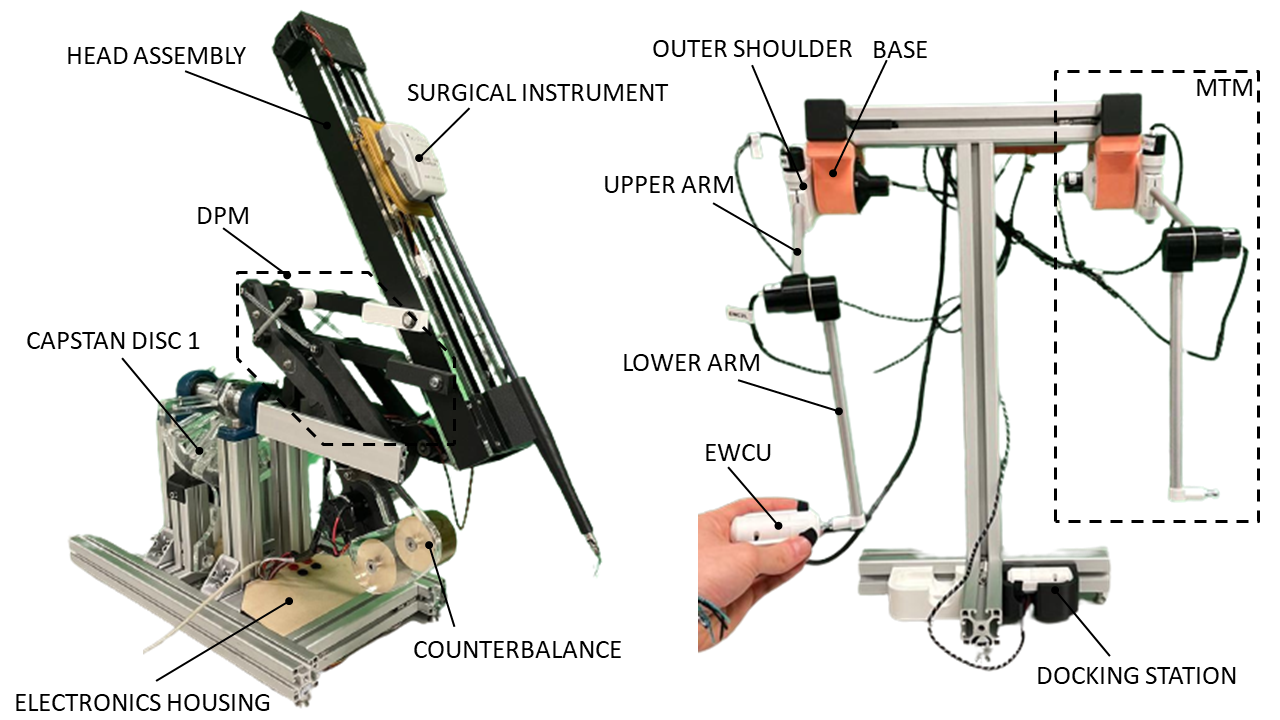
\includegraphics[width=.750\linewidth]{figures/system_overview.png}
    \caption{ Overview of the Desktop Teleoperated Surgical Training System, illustrating the MTM and PSM components.}
    \label{fig:system_overview} % Renamed label for consistency
\end{figure}


\subsection{MTM Overview}

The MTM is a serial-link manipulator that measures the operator's motion through a 7-DOF linkage, actuated by the user. The associated DOFs and their types are indicated in Table~\ref{tab:mtm_dofs_detailed}.

\begin{table}[H] 
    \caption{MTM Joint Classification and Positional Sensing.}
    \label{tab:mtm_dofs_detailed}
    \begin{tabular}{|l|l|l|}
    \hline
    \textbf{Joint Classification} & \textbf{Dof Name} & \textbf{Positional sensing} \\
    \hline
    \multirow{3}{*}{\raggedright Overall system positioning} & J0 & \multirow{3}{*}{12-bit absolute magnetic encoder} \\
    & J1 & \\
    & J2 & \\
    \hline
    \multirow{4}{*}{\raggedright Instrument positioning} & G0 & Hall Effect Sensor \\
    \cline{2-3}
    & G1 & \multirow{3}{*}{Analog Potentiometer} \\
    & G2 & \\
    & G3 & \\
    \hline
    \end{tabular}
\end{table}
These joints allow the operator to communicate desired motions to the PSM. The J0--J2 DOFs dictate the endpoint position, while G0--G3 control endpoint orientation and state.

The MTM should allow for accurate interpretation of the operator's intended motion while also minimizing the force perceived by the operator. This perceived force requirement drove the design toward a gravity compensation system (GCS).

An overview of the MTM with indications to the specific DOFs can be seen in Figure~\ref{fig:mtm_dofs}.

\begin{figure}[H] % Changed from [H] for better float placement
    \centering
    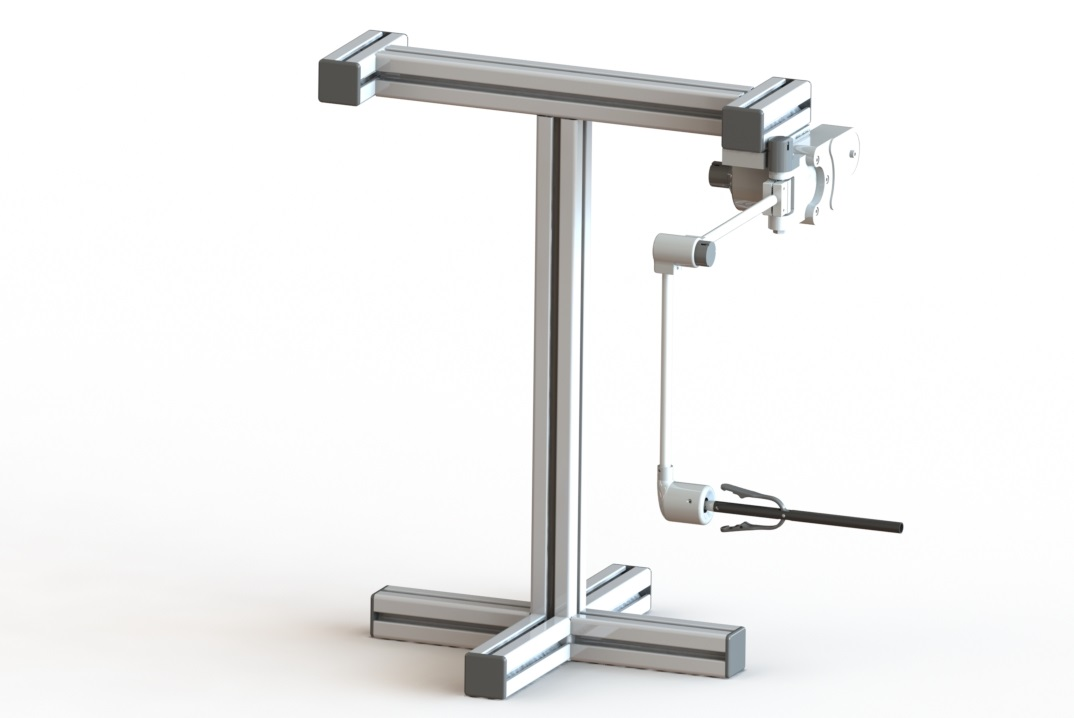
\includegraphics[width=.6\linewidth]{figures/MTMOverview.png} % Adjust width as needed
    \caption{Overview of the MTM with indicated DOFs.}
    \label{fig:mtm_dofs}
\end{figure}

\subsection{PSM Overview}

The PSM has 7 primary DOFs, classified as shown in Table~\ref{tab:psm_dofs}.


\begin{table}[H]
    \caption{PSM Joint Classification and Drive System.}
    \label{tab:psm_dofs}
    \setlength{\tabcolsep}{4pt} % Adjust this value (e.g., 2pt, 4pt) to fine-tune column spacing
    \begin{tabular}{|p{3.0cm}|l|l|p{4.5cm}|} % Changed p{} to l for left-justification where needed
    \hline
    \textbf{Joint Class} & \textbf{DOF Name} & \textbf{Drive Type} & \textbf{Positional sensing} \\
    \hline
    \multirow{3}{3.0cm}{\raggedright Overall system positioning} & Roll & \multirow{3}{*}{Brushless DC Motor} & \multirow{3}{4.5cm}{\raggedright 12-bit absolute magnetic encoders} \\
    & Pitch & & \\
    & Insertion & & \\
    \hline
    \multirow{4}{3.0cm}{\raggedright Instrument positioning} & Instrument Roll & \multirow{4}{*}{Servo Motor} & \multirow{4}{4.5cm}{\raggedright Servo feedback} \\
    & Instrument Pitch & & \\
    & Instrument Tilt & & \\
    & Instrument Grasp & & \\
    \hline
    \end{tabular}
\end{table}


An overview of the system with indications to the specific DOFs can be seen in Figure~\ref{fig:psm_overview}.

\begin{figure}[H] % Changed from [H] for better float placement
    \centering
    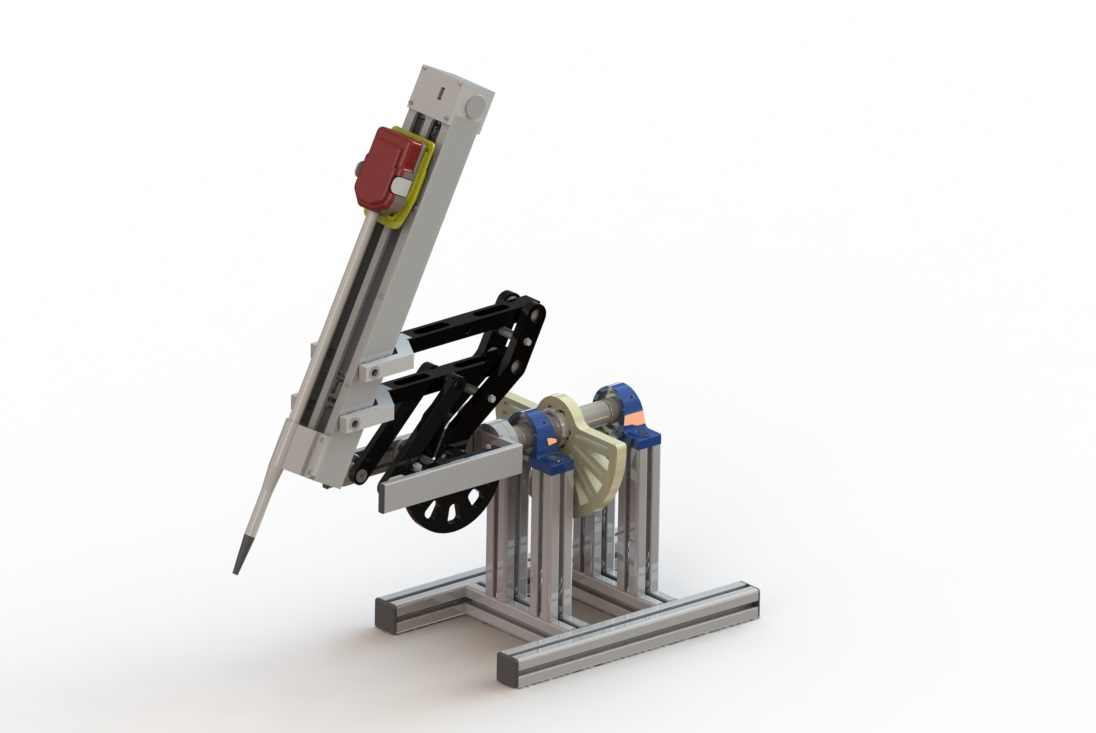
\includegraphics[width=0.6\linewidth]{figures/PSMOverview.png} 
    \caption{Overview of the PSM with indicated DOFs.}
    \label{fig:psm_overview}
\end{figure}

\section{Master Tool Manipulator Mechanical Design}

The Master Tool Manipulator (MTM) mechanical design can be separated into three subsystems, the arm (J0-J2), the gimbal (G0-G3) and the superstructure.

The arm subsystem is the primary architecture responsible for measuring the operator's position relative to the global reference frame. Three revolute joints with internal absolute magnetic encoders are coupled via rigid aluminum extrusions, allowing accurate estimation of the overall system positioning in 3D space.

The Gimbal subsystem, which is responsible for measuring the desired surgical instrument inputs, is a self-contained, 4-axis analog sensing apparatus. A 3D-printed shell contains the necessary analog sensing devices for determining the desired wrist position.

The superstructure is an aluminum extrusion structure that offsets the arm and gimbal subsystems from the table to allow space for manipulation. An overview of the design of the MTM, with indications to each subsystem, can be seen in Figure~\ref{fig:mtm_overview}.

\begin{figure}[H] % Changed from [h!] for better float placement
    \centering
    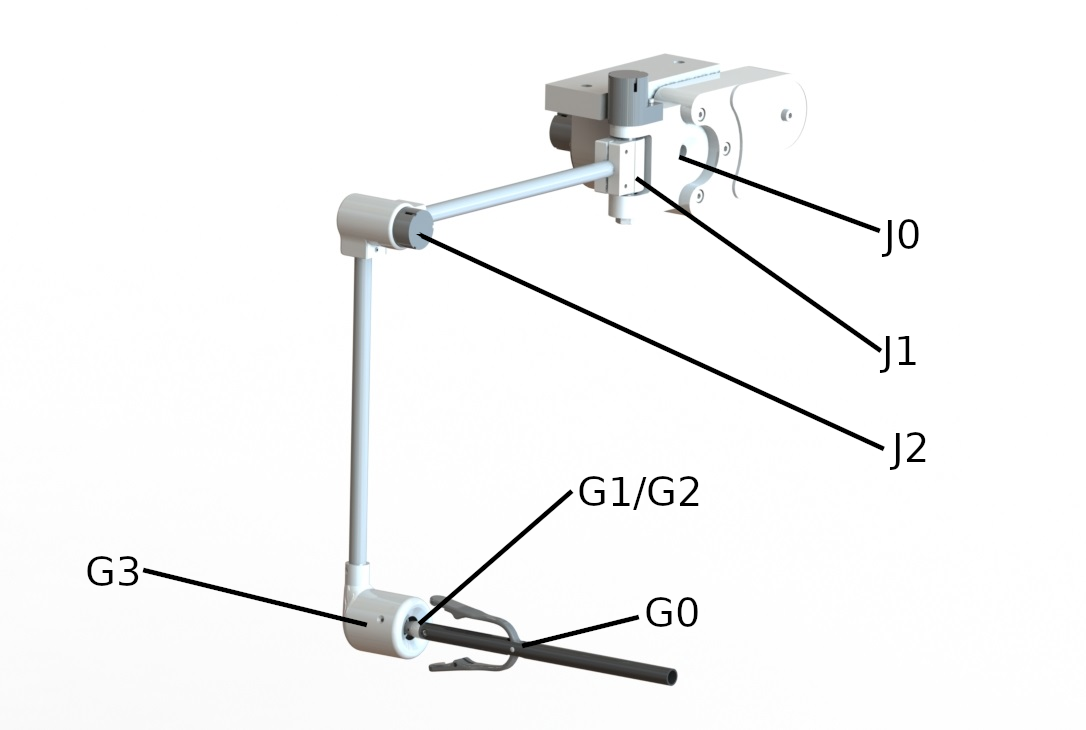
\includegraphics[width=1.0\linewidth]{figures/ArmOverview.png}
    \caption{Overview of the entire MTM system with indications to the subsystems.}
    \label{fig:mtm_overview}
\end{figure}

\subsection{Superstructure Design}

The superstructure design is relatively straightforward. With no moving parts, it is purely designed to offer a platform on which the more complicated mechanics of the MTM can be mounted.

Several pieces of 20mm x 20mm aluminum extrusion are bolted together, offering a stable and modular platform. Previously, a 3D-printed piece held an Arduino Mega at the top of the superstructure, but this was updated to hold a Teensy 4.1 on the main superstructure beam to allow for easier access and wiring. 

\subsection{Arm Joint Design}

The arm joints of the MTM feature relatively straightforward designs. The arm subsystem is rigidly coupled to the superstructure with a 3D-printed block, to which the origin of the arm's J0 joint is connected. Each joint is a simple revolute joint, directly coupled to an EAT-6012-A06 12-bit absolute magnetic encoders. These joints are then rigidly connected to each other through aluminum tubing, held in place by set screws. A detailed exploration of the J1 joint can be seen in Figure~\ref{fig:J1_detailed}. 

\begin{figure}[H] 
    \centering
    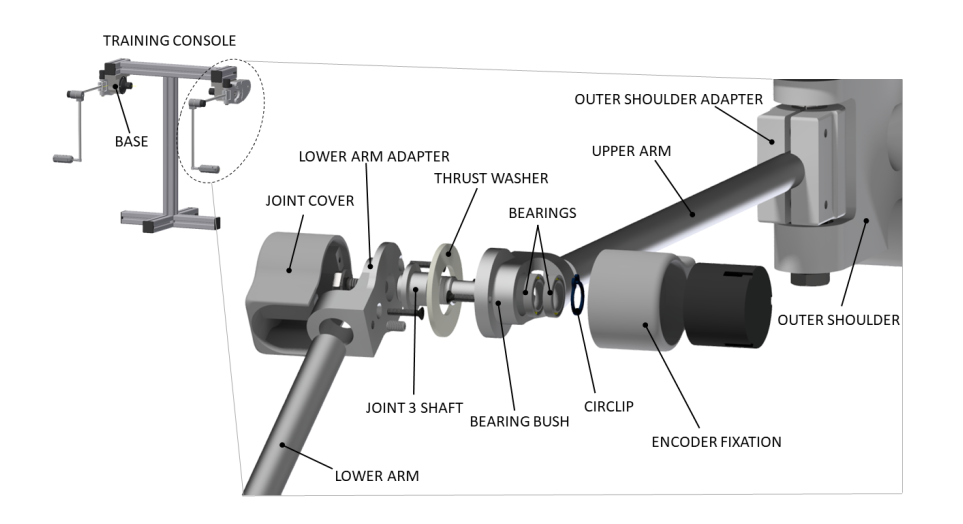
\includegraphics[width=1.00\linewidth]{figures/J1_detailed.png} 
    \caption{Detailed view of the MTM's J1 joint design (Reprinted from \cite{walder2022design} Fig 2.1)} 
    \label{fig:J1_detailed} 
\end{figure}

The design of these joints was driven by the requirement to minimize friction. Increased frictional forces in any of these joints would result in an increase in perceived force by the operator. Roller bearings were utilized to minimize these frictional forces, and system mass was also reduced to lower both gravitational and inertial forces felt by the operator. However, in an effort to completely minimize forces felt by the operator, a GCS was implemented into the J0 joint.

The GCS consists of a brass cylinder, carefully massed to offset the gravitational forces felt by the system. The exact placement and mass of this cylinder were algorithmically determined in \cite{walder2022design} A detailed view of the mechanical design of this system can be seen in Figure~\ref{fig:GCS_detailed}.

\begin{figure}[H] % Changed from [H] for better float placement
    \centering
    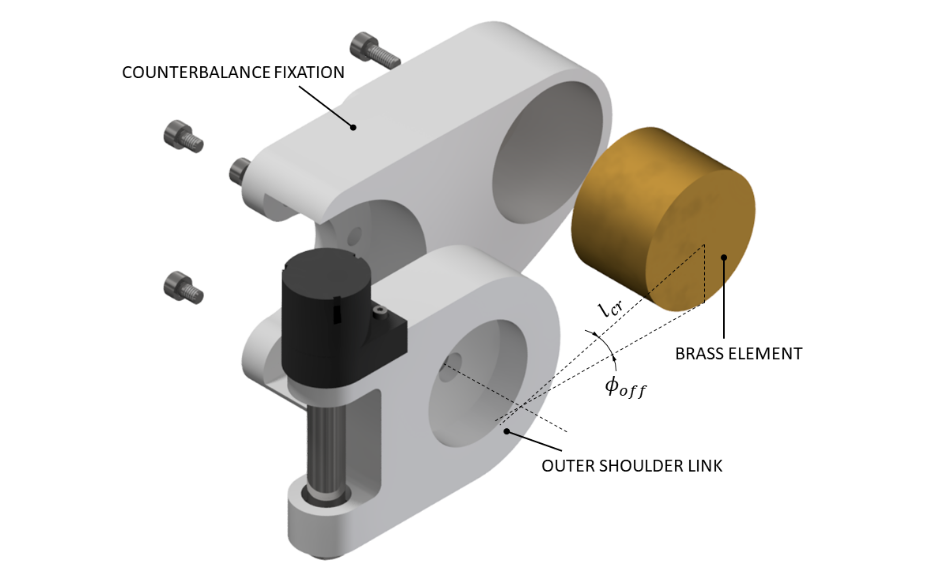
\includegraphics[width=1.0\linewidth]{figures/GCS_detailed.png}
    \caption{Detailed overview of the MTM's GCS design. (Reprinted from \cite{walder2022design} Fig 2.9)}
    \label{fig:GCS_detailed}
\end{figure}

\section{MTM Electrical Architecture}


\subsection{System Overview}
The MTM electrical architecture was originally based on an Arduino Mega 2560 microcontroller, which served as both the primary controller and system I/O interface. This configuration was later upgraded to a Teensy 4.1 microcontroller due to its superior performance and compatibility with ROS2 and micro-ROS frameworks.

The system incorporates multiple sensor subsystems to monitor and control the robotic arm's movements. Each DOF of the MTM is equipped with its own independent sensor for full positional sensing.

\subsection{Joint Subsystems}
Joints J0-J2 are equipped with AEAT-6012-A06 12-bit absolute magnetic encoders (resolution: 4096 counts/revolution) directly coupled to each joint axis. These encoders provide a positional accuracy of $\pm 0.088^\circ$ ($360^\circ/4096$) per joint, enabling precise positional feedback for the control system. The encoder signals are connected directly to the Teensy 4.1's digital I/O pins and are supplied 5V power directly from the Teensy 4.1.

\subsection{Gimbal Subsystem}
The wrist subsystem underwent significant design evolution. Initially, the wrist sensing utilized an MPU-6050 3-DOF IMU coupled with a Hall effect sensor for full positional sensing of the wrist subsystem \cite{Preiss2022Haptically}. However, during the course of this research, this subsystem was updated to replace the IMU with a series of three potentiometers coupled to a Hall effect sensor. G0 is measured using a Hall effect sensor on a lever arm linkage. This is then coupled to a modified FJN10K-C0 two-axis joystick potentiometer, which handles the angular sensing of G1 and G2. This joystick is coupled to the G3 potentiometer through a 3D-printed linkage. G0 used a SS495A Hall Effect Sensor, G1/G2 used a FJN10K-C0 two-axis joystick potentiometer, and G3 used a 3382H-1-103 Potentiometer.

Each of these sensors is supplied 3.3V power from the Teensy 4.1, and their resultant analog signals are sent to the Teensy 4.1's analog input pins.

\section{PSM Mechanical Design}

\subsection{Overview}
The Patient-Side Manipulator mechanical architecture is a 7-degree-of-freedom robotic system designed to replicate surgical instrument movements with high precision. The design is fundamentally inspired by the da Vinci Surgical System's remote center of motion mechanism, which maintains a fixed pivot point at the surgical incision site - a critical feature for minimally invasive surgery. The PSM can be divided into five primary subsystems., Superstructure and base, Roll axis, Pitch axis, Insertion axis, and Tool cart and end effector.

\subsection{Superstructure}
The superstructure serves as the foundational framework, constructed from 80/20 aluminum extrusion for both rigidity and modularity. The base of the superstructure also houses the necessary electronics for the control of the PSM. 

\subsection{Roll Axis}
The roll axis implements a revolute joint providing $\pm 30^\circ$ of rotation about the vertical axis. The system rotates in two roller bearings attached to the superstructure with a Commercial Off-The-Shelf bearing block. A laser-cut acrylic wheel serves as the capstan drive of the system and is clamped to the central shaft. This wheel is connected to a brushless DC motor via steel cabling, offering a 20:1 reduction in a zero-backlash setup. This shaft terminates in a forked aluminum extrusion structure, to which the pitch subsystem connects. A limit switch is attached to the superstructure to allow for zeroing of the system.

This design offered a simple way to achieve precise, zero-backlash performance in an easy-to-assemble and low-cost package. A detailed depiction of this subsystem can be seen in Figure~\ref{fig:roll_detailed}.

\begin{figure}[H] % Added placement specifier
    \centering
    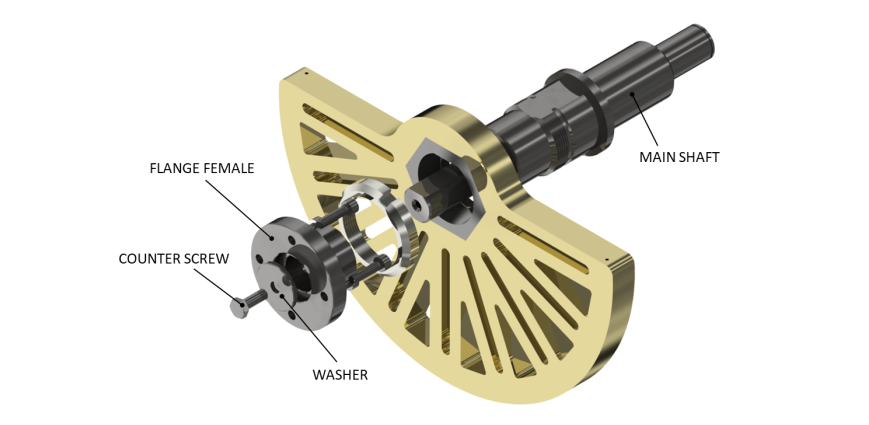
\includegraphics[width=1.0\linewidth]{figures/roll_detailed.png}
    \caption{Detailed view of the mechanical design of the roll axis, highlighting the main shaft design. (Reprinted from \cite{walder2022design} Fig 2.10)}
    \label{fig:roll_detailed}
\end{figure}

To minimize forces seen by the actuator, a gravity compensation system (GCS) was applied to this joint. This GCS consisted of two adjustable brass counterweights hanging directly below the capstan drive. Their mass and placement were once again algorithmically determined by previous research conducted by Walder \cite{walder2022design}. A detailed view of the design of this GCS can be seen in Figure~\ref{fig:PSM_GCS}.

\begin{figure}[H] % Added placement specifier (requires \usepackage{float} if using [H], but [htb!] is generally better)
    \centering
    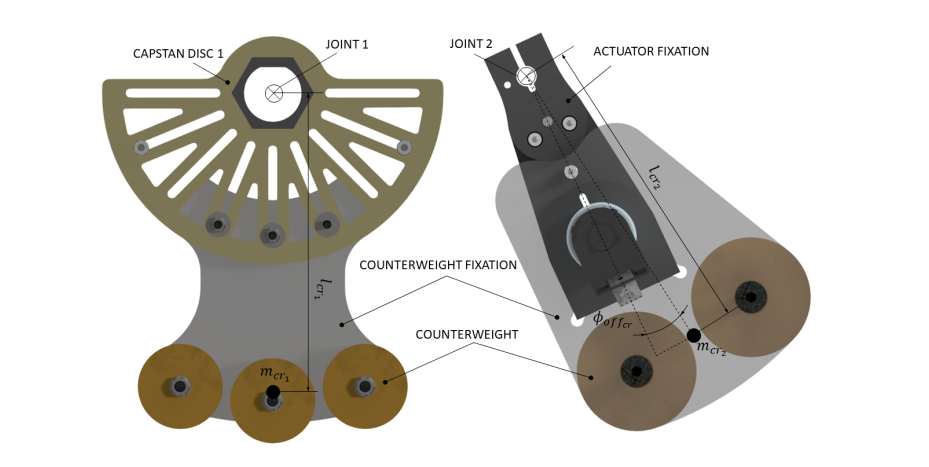
\includegraphics[width=0.75\linewidth]{figures/PSM_GCS.png}
    \caption{A detailed view of the PSM's pitch and roll GCS design. (Reprinted from \cite{walder2022design} Fig. 2.22)}
    \label{fig:PSM_GCS}
\end{figure}


\subsection{Pitch Axis}
The pitch axis replicates the Da Vinci's characteristic double parallelogram mechanism, which creates a virtual RCM distal to the joint. For ease of manufacturing, much of the PSM's pitch subsystem was designed to be 3D-printed, and for ease of assembly, many of the couplings were press-fits. This led to sagging of the mechanism and resulted in some of the linkages requiring maintenance during prolonged operation, but, overall, the linkage design was sound and maintained a remote center.

The pitch axis was coupled to the roll axis through the forked aluminum extrusion structure previously discussed in the PSM mechanical design section. Similar to the roll axis, the pitch axis was driven by a capstan drive system coupled to a brushless DC motor through steel cabling. A limit switch at the extreme limits of motion was once again used for zeroing the system, and the mechanism ultimately resulted in a $\pm 30^\circ$ range of motion. A detailed view of the pitch subsystem design can be seen in Figure~\ref{fig:pitch_detailed}.

Once again, a GCS was designed for the pitch subsystem. This design followed similar trends to the roll axis, placing a brass counterweight below the axis to reduce the force seen by the actuator. The design of this can be seen in Figure~\ref{fig:PSM_GCS}. 


\begin{figure}[H]
    \centering
    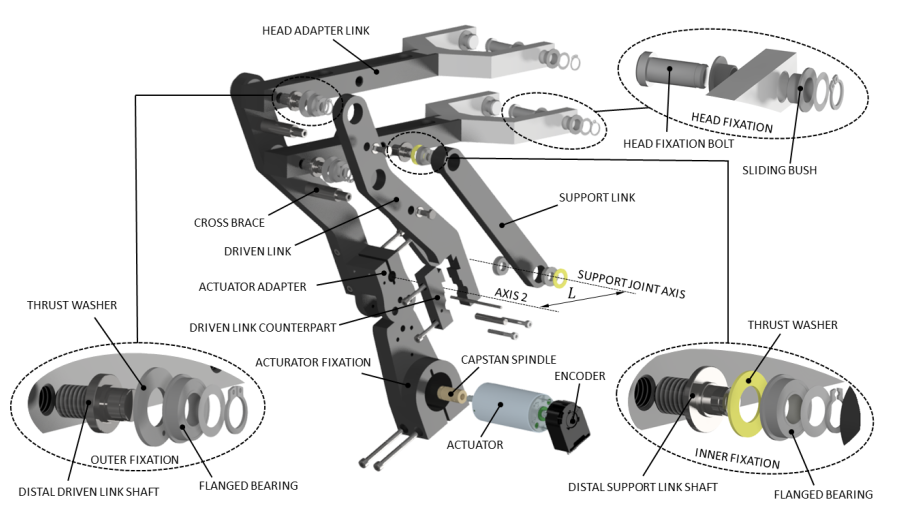
\includegraphics[width=1.0\linewidth]{figures/pitch_detailed.png}
    \caption{Detailed view of the PSM's pitch axis mechanism. (Reprinted from \cite{walder2022design} Fig 2.13)}
    \label{fig:pitch_detailed}
\end{figure}

\subsection{Insertion Axis}

The insertion axis design is relatively straightforward. A brushless DC motor coupled directly to a rack and pinion mechanism translates the rotary motion of the motor into the linear motion needed for the insertion axis. For ease of manufacturing, the majority of this mechanism was 3D-printed, and it was coupled to the pitch subsystem through a bolted connection via the end forks of the pitch linkage. For positional sensing, the carriage was coupled to an encoder through a belted connection. A detailed diagram of this subsystem can be seen in Figure~\ref{fig:insertion_detailed}.

\begin{figure}[H]
    \centering
    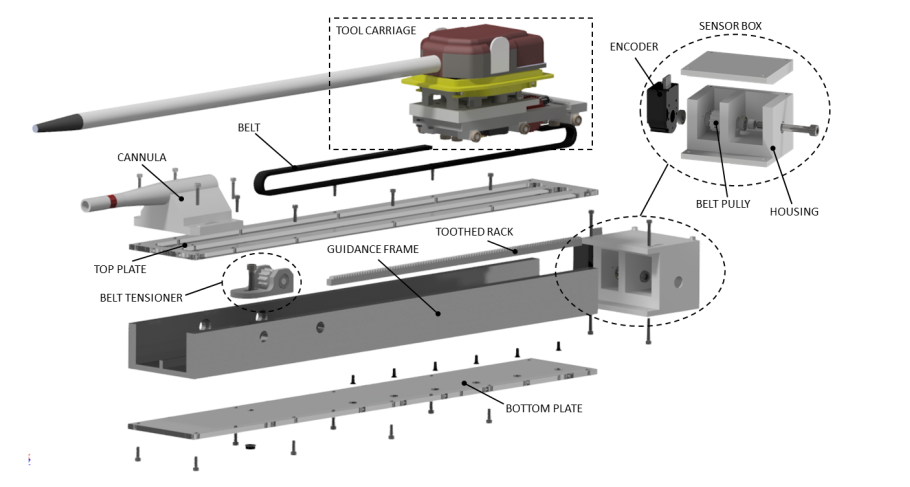
\includegraphics[width=1.0\linewidth]{figures/insertion_detailed.png}
    \caption{Detailed view of the PSM's insertion axis mechanism. (Reprinted from \cite{walder2022design} Fig 2.14)}
    \label{fig:insertion_detailed}
\end{figure}

\subsection{Tool Cart and End Effector}
The tool cart is responsible for driving the surgical instrument. This system uses off-the-shelf Intuitive Surgical instruments. These instruments are driven by a belted disc mechanism internal to the instrument. The tool cart houses four servo motors coupled to these discs with a spring-loaded compliance mechanism, as shown in Figure~\ref{fig:tool_cart_detailed}.

\begin{figure}[H]
    \centering
    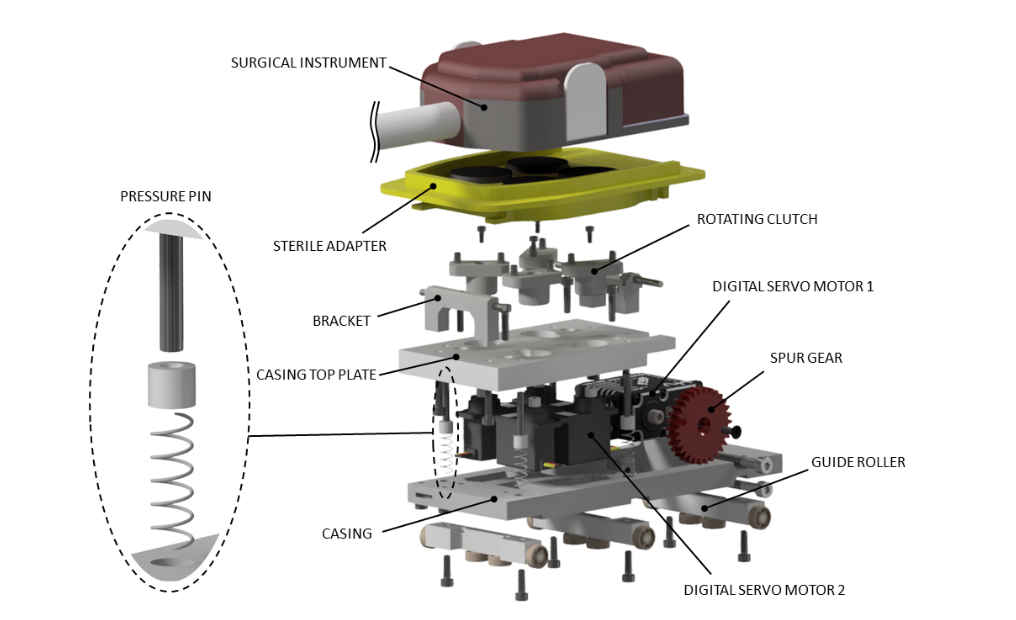
\includegraphics[width=1.0\linewidth]{figures/tool_cart_detailed.png}
    \caption{Detailed view of the PSM's tool cart, highlighting the spring-loaded compliance mechanism. (Reprinted from \cite{walder2022design} Fig 2.15)}
    \label{fig:tool_cart_detailed}
\end{figure}



\section{PSM Electrical Architecture}

The PSM electrical architecture is based on a Teensy 4.1 as the control unit of the system. Table~\ref{tab:psm_specs} showcases each joint's associated electrical components.

\begin{table}[htb!]
    \centering
    \caption{PSM Joint Specifications} % You can adjust the caption as needed
    \label{tab:psm_specs} % You can adjust the label as needed
    % p{0.15\linewidth} for Joint column (approx 15% of text width)
    % p{0.25\linewidth} for Drive Motor (approx 25%)
    % p{0.25\linewidth} for Motor Driver (approx 25%)
    % p{0.27\linewidth} for Positional Sensing (approx 27%)
    % Total width ~0.92\linewidth, leaving some margin.
    \begin{tabular}{|p{0.15\linewidth}|p{0.25\linewidth}|p{0.25\linewidth}|p{0.27\linewidth}|}
        \hline
        \textbf{Joint} & \textbf{Drive Motor} & \textbf{Motor Driver} & \textbf{Positional Sensing} \\
        \hline
        Pitch & \multirow{3}{=}{\centering Maxon 273752 15V DC motor} & \multirow{3}{=}{\centering MD13S Cytron 13 Amp} & \multirow{3}{=}{\centering Broadcom HEDS-5540 encoder} \\
        Roll & & & \\
        Insertion & & & \\
        \hline
        Tool Roll & \multirow{4}{=}{\centering MG966r Servo} & \multirow{4}{=}{\centering None} & \multirow{4}{=}{\centering Servo Feedback} \\
        Tool Tilt & & & \\
        Tool Pitch & & & \\
        Tool Grasp & & & \\
        \hline
    \end{tabular}
\end{table}

\section{System Software Architecture}
\label{sec:software_architecture}

As noted earlier in this paper, the initial software framework was implemented in an Arduino C-based environment. While the system has since been migrated to a ROS 2 architecture, the original implementation remains relevant for context and reference.

The software was divided into two primary components: the MTM software and the PSM software. These subsystems worked in tandem to enable real-time teleoperation, with the MTM capturing user inputs and the PSM replicating movements precisely.

\subsection{MTM Software}
The MTM software was responsible for several critical functions. Sensor data was read and processed from each of the DOFs associated sensors. Data was then filtered and converted into angular measurements based on predefined system parameters. Forward kinematics were then used to calculate the end effectors position based on angular measurements from sensors. Denavit-Hartenberg (DH) parameters were used for the forward kinematic calculations. All of the associated MTM data had to be parsed into a single serial string and output to the serial monitor for later acquisition by the PSM. In addition, sensor overflow was carefully monitored and spike detection logic was implemented to catch any spikes in sensor data. All relevant data had to be packaged with start/end markers for easy access and parsing by the PSM.


\subsection{PSM Software}
The PSM software was responsible for the control and drive of the PSM based on the movements of the MTM. Upon receiving target data from the MTM through the serial monitor the data had to be parsed and processed using a custom parsing function. The target position was then extracted from this data. Each joint was controlled through a PID control function with predetermined gains. Each joint had to be homed to its 0 position and the absolute encoder 0 value was also set through a ramp-up homing sequence in which the system carefully managed joint speed as it approaches the limit of motion.
During operation limit switch state was monitored to ensure each joint was not colliding with the mechanical hard-stops. To ensure the surgical tool discs were engaged a tool catch procedure ran each servo through its complete range of motion and the PWM frequency was set to ensure that it lie outside of human range of hearing.

\section{System Controller Design}

Previous research conducted on the platform resulted in a basic controller design. Initially, a Proportional-Integral-Derivative (PID) controller was designed using the Ziegler-Nichols method. This approach involved determining the critical gain ($K_{cr}$) and periodic time ($P_{cr}$) for each joint through root locus analysis, identifying where the dominant poles intersected the imaginary axis. These values were then used with the McCormack tuning rules to calculate the initial PID constants, as presented in Table \ref{tab:pid_constants}.

\begin{table}[h!]
    \centering
    \caption{Initial PID Constants}
    \label{tab:pid_constants}
    \begin{tabular}{lccc}
        \toprule
        \textbf{Joint} & \textbf{Proportional gain ($K_p$)} & \textbf{Integral gain ($K_i$)} & \textbf{Derivative gain ($K_d$)} \\
        \midrule
        Roll & 35.0 & 50.0 & 5.0 \\
        Pitch & 60.0 & 110.0 & 15.0 \\
        Insertion & 45.0 & 800.0 & 3.8 \\
        \bottomrule
    \end{tabular}
\end{table}

However, initial trials with these derived parameters revealed significant overshoot, unacceptably long settling times, and the system frequently entered uncontrolled oscillations. As a result of these shortcomings, manual tuning of the PID coefficients was required to achieve satisfactory performance. Nevertheless, even these manually tuned PID gains still resulted in unstable oscillations, particularly at the extreme ends of the range of motion. Consequently, the system was often operated using a simple P controller with manually selected gains, leading to very poor overall system performance.


\section{System Kinematics and Coordinate Frames}

It is critical to understand the system kinematics and coordinate frames for this system. This section will illustrate the defined coordinate frame positions with the system in its respect 0 positions. 

\subsection{MTM Coordinate Frame}

As stated earlier, the MTM has 7 degrees of freedom. It is imperative to understand the coordinate frame of each of these axes. Figure \ref{fig:MTMcoords} showcases each of these axes in their zero position with their respective coordinate frames attached. A detailed view of the updated gimbal design with each of the axes in their zero position can be seen in Figure~\ref{fig:GimbalCoords}.

\begin{figure}[H]
    \centering
    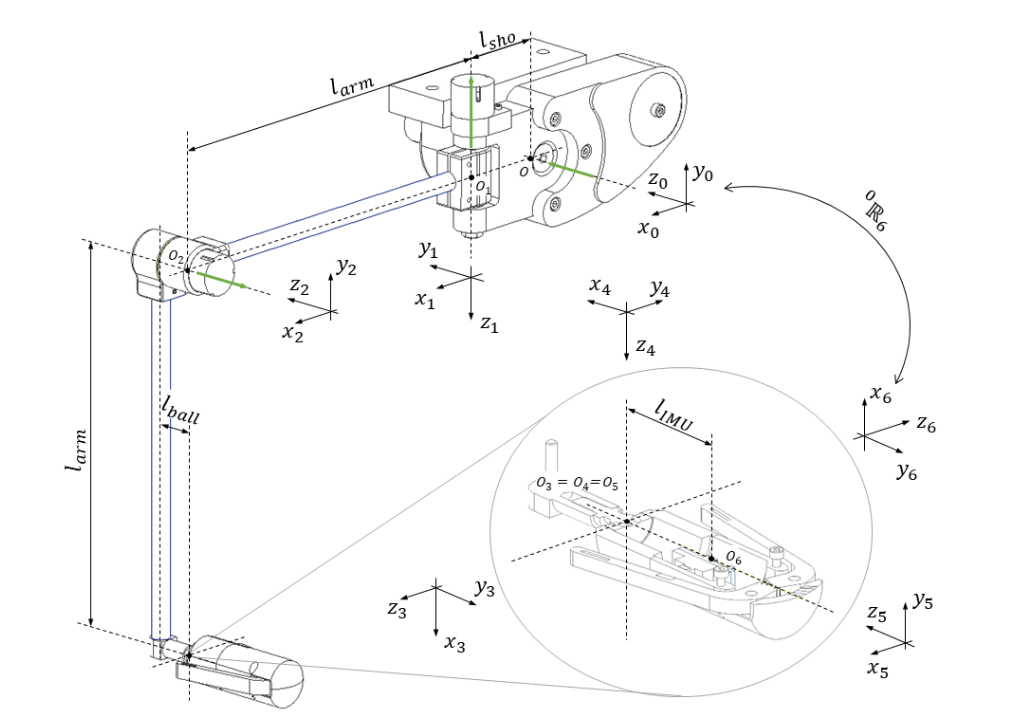
\includegraphics[width=0.7\linewidth]{figures/MTMcoords.png}
    \caption{The MTM and its associated degrees of freedom shown in their zero-position with DH-coordinate frames attached (Reprinted from \cite{walder2022design} Fig 3.1)}
    \label{fig:MTMcoords}
\end{figure}

\begin{figure}[H]
    \centering
    \includegraphics[width=0.7\linewidth]{figures/Gimbalcoords.png}
    \caption{The updated gimbal and its associated degrees of freedom shown in their zero-position.  (Reprinted from \cite{Messner2025Teleoperative} Fig 2.1)}
    \label{fig:GimbalCoords}
\end{figure}

\subsection{PSM and Tool Coordinate Frame}

The PSM and its associated tool have a total of 7 degrees of freedom. Each of these degrees of freedom can be seen in their zero position in \textbf{Figure \ref{fig:PSMCoord}}.

\begin{figure}[htb!]
    \centering
    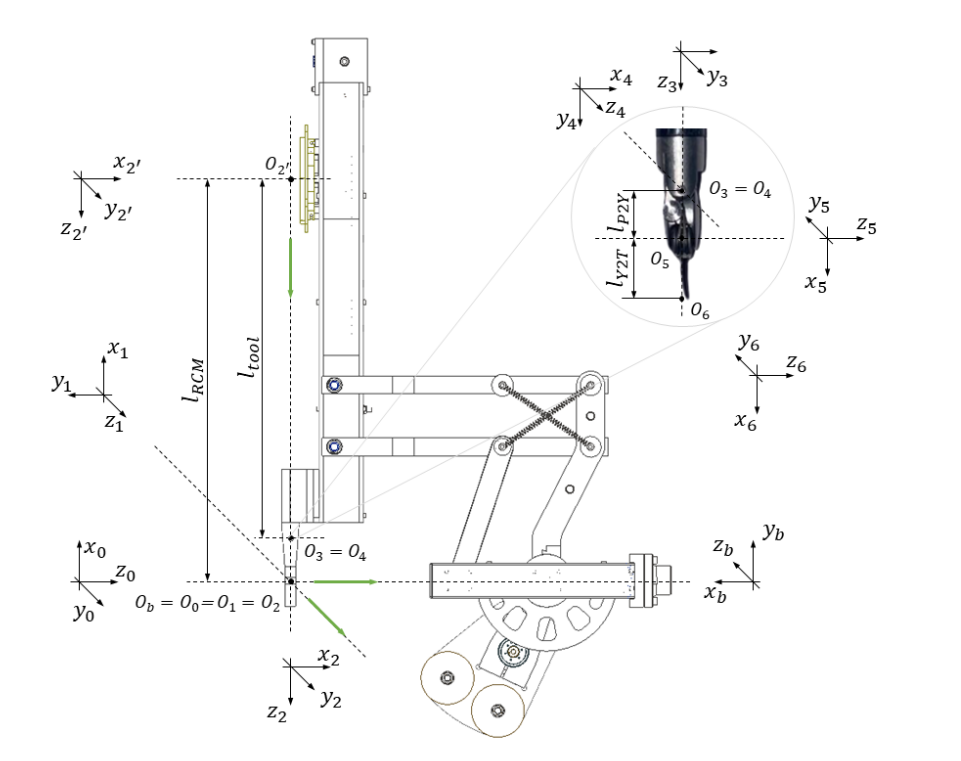
\includegraphics[width=1.0\linewidth]{figures/PSMcoord.png}
    \caption{The PSM and endowrist tool shown in their zero-position with DH-coordinate frames attached, according to the cDH convention. (Reprinted from \cite{walder2022design} Fig 3.2)}
    \label{fig:PSMCoord}
\end{figure}
\chapter{Implementation on Current Hardware}

\section{Software Architecture}

This section will serve as an overview of the current system software architecture and will provide an in-depth analysis of how the current ROS 2 Node structure works.

\subsection{ROS 2 System Architecture}

The system's ROS 2 architecture was composed of 4 primary software nodes. The MTM node was responsible for streaming sensor data from the MTM, while also calculating joint angles and relaying these angles to the joint publisher node. The system model node consisted of an SDF model of the MTM allowing for visualization of the MTM's position. Additionally, target end effector position could be calculated from this model through frame transformations. The joint publisher node acted as intermediate between the SDF model and the ROS 2 workspace. It relayed the joint angles from the MTM to the SDF model and the target end effector position to the the PSM node. Finally, the PSM node was responsible for the control and drive of the PSM. It also broadcasted PSM sensor data and joint states into the ROS2 workspace.

\begin{figure}[h!]
    \centering
    \begin{tikzpicture}[node distance=1cm, auto] % Reduced node distance for a narrower figure
        % Nodes
        \node (mtm) [block] {MTM Node};
        \node (sdf) [block, right=of mtm] {SDF Model};
        \node (jointpub) [block, right=of sdf] {Joint Publisher Node};
        \node (psm) [block, right=of jointpub] {PSM Node};

        % Arrows
        \draw[arrow] (mtm) -- (sdf);
        \draw[arrow] (sdf) -- (jointpub);
        \draw[arrow] (jointpub) -- (psm);
    \end{tikzpicture}
    \caption{Initial ROS 2 System Architecture for Target Pose Calculation.}
    \label{fig:initial_architecture}
\end{figure}

Initially, the research aimed for the MTM Node to relay its joint angles to the SDF Model of the MTM. Subsequently, the Joint Publisher Node would calculate the desired end-effector position via a TF frame transformation from the base frame to the gimbal origin. This approach was intended to provide an alternative method for extracting the target position, bypassing the need for explicit forward kinematics in the MTM node. This architecture is illustrated in Figure \ref{fig:initial_architecture}. While this method proved effective in accurately calculating the target pose, real-time performance trials revealed significant limitations.

Specifically, while target position extracted from the model demonstrated excellent real-time performance, a communication issue was found when the Joint Publisher Node interfaced with the PSM Node. This breakdown was likely caused by memory limitations in the Teensy 4.1, leading to high latency and noticeable data stuttering.

As a result, a simplified architecture was briefly explored to try to prevent this issue. This approach directly calculated the target pose using forward kinematics in the MTM node and then directly relayed this to the PSM node. This simplification of the technical stack had the potential to increase real-time performance; however, it also increased the forward kinematics calculation complexity and eliminated the opportunity to use the SDF model for further research. This architecture is presented in Figure \ref{fig:optimized_architecture}.

\begin{figure}[h!]
    \centering
    \begin{tikzpicture}[node distance=2.5cm, auto]
        % Nodes
        \node (mtm) [block] {MTM Node};
        \node (psm) [block, right=of mtm] {PSM Node};

        % Arrows
        \draw[arrow] (mtm) -- (psm);
    \end{tikzpicture}
    \caption{Simplified ROS 2 System Architecture for Direct Target Pose Streaming.}
    \label{fig:optimized_architecture}
\end{figure}

Ultimately, this simplified architecture was not chosen. The elimination of the SDF model would result in limitation of future research resources and as a result the initial architecture was chosen, and further development efforts were undertaken to eliminate the data loss issues previously discussed.

\subsection{MTM Modeling and Visualization}

For the modeling of the MTM, the Simulation Description Format (SDF) was chosen due to its compatibility with ROS 2 and RViz. SDF also supports complex kinematic structures, including closed-chain kinematics, which is crucial for accurately modeling the more intricate four-bar style linkages found in the PSM.

Generating the SDF file proved to be a fairly involved process. First, the CAD model of the MTM system was imported into SolidWorks. To reduce computational complexity, the model underwent significant simplification. Parts were condensed into their respective links, identified as Base, J1 (Joint 1), J2 (Joint 2), J3 (Joint 3), G3 (Gimbal Link 3), G2 (Gimbal Link 2), G1 (Gimbal Link 1), and G0 (Gimbal Link 0).
Each of these components was created as a singular solid part and then reassembled within SolidWorks into a complete assembly.

Following this, rotational axes and origins were assigned for each link. A SolidWorks plugin was then utilized to export the model into a Universal Robot Description Format (URDF) file \cite{ROS:SWURDFExporter}. This URDF file was subsequently converted to SDF using \textit{ros2\_sdf\_to\_urdf} \cite{BruceChanJianLe:igngzu_urdf_to_sdf}. Upon the successful generation of the SDF model, a Python launch file was developed to facilitate quick and easy visualization of this model within RViz.

The final result of this effort can be seen below in Figure \ref{fig:mtm_sdf_model}.

\begin{figure}[H]
    \centering
    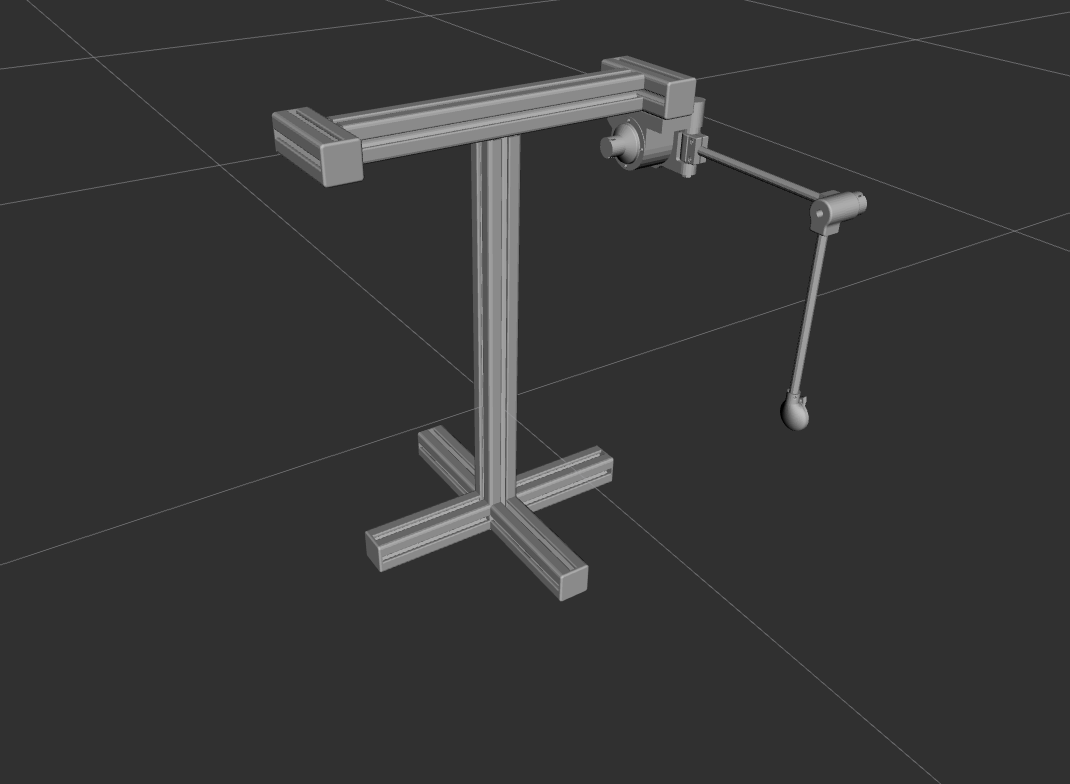
\includegraphics[width=0.9\linewidth]{figures/mtm_sdf_model.png}
    \caption{SDF model of MTM shown in the RViz environment. The gimbal solid models have been hidden in this model}
    \label{fig:mtm_sdf_model}
\end{figure}

\subsection{MicroROS Implementation}

Since the teensy 4.1 does not support the full ROS 2 stack, MicroROS was utilized to allow the microcontroller to communicate with the ROS 2 system. MicroROS is a lightweight version of ROS 2 designed for microcontrollers and resource-constrained devices. It provides a subset of the ROS 2 features, enabling communication between nodes while maintaining low memory and processing overhead. 

In order to set up MicroROS on the Teensy 4.1, the following procedure was implemented in both the MTM and PSM nodes to initalize the MicroROS environment:

First the necessary Micro-ROS header was included
\begin{lstlisting}[language=C++, caption={Include Micro-ROS PlatformIO Header}, label={lst:microros_include}]
#include <micro_ros_platformio.h>
\end{lstlisting}

Next, the serial port was configured as the communication transport for Micro-ROS.

\begin{lstlisting}[language=C++, caption={Set Micro-ROS Serial Transport}, label={lst:microros_serial_transport}]
Serial.begin(921600);
set_microros_serial_transports(Serial);
delay(2000); // Give time for connection to establish
\end{lstlisting}

The default allocator was obtained and used for memory management.
\begin{lstlisting}[language=C++, caption={Initialize Micro-ROS Allocator}, label={lst:microros_allocator}]
allocator = rcl_get_default_allocator();
\end{lstlisting}

The \texttt{rclc\_support\_init} function initialized the Micro-ROS support structure, which is a key ROS 2 component
\begin{lstlisting}[language=C++, caption={Initialize Micro-ROS Support Structure}, label={lst:microros_support_init}]
RCCHECK(rclc_support_init(&support, 0, NULL, &allocator));
\end{lstlisting}

Next a ROS 2 node was created 
\begin{lstlisting}[language=C++, caption={Initialize ROS 2 Node}, label={lst:microros_node_init}]
RCCHECK(rclc_node_init_default(&node, "mtm_arm_node", "", &support));
\end{lstlisting}

All necessary publisher were created to send messages on specified topics
\begin{lstlisting}[language=C++, caption={Initialize Micro-ROS Publishers}, label={lst:microros_publishers}]
RCCHECK(rclc_publisher_init_default(
  &joint_state_publisher,
  &node,
  ROSIDL_GET_MSG_TYPE_SUPPORT(sensor_msgs, msg, JointState),
  "mtm_joint_states"));

RCCHECK(rclc_publisher_init_default(
  &raw_values_publisher,
  &node,
  ROSIDL_GET_MSG_TYPE_SUPPORT(std_msgs, msg, Float32MultiArray),
  "mtm_raw_values"));

RCCHECK(rclc_publisher_init_default(
  &target_pose_publisher,
  &node,
  ROSIDL_GET_MSG_TYPE_SUPPORT(sensor_msgs, msg, JointState),
  "/target_pose"));
\end{lstlisting}

Finally, the Micro-ROS executor was initialized. The executor is responsible for managing the execution of callbacks associated with subscriptions, timers, and other ROS 2 entities.
\begin{lstlisting}[language=C++, caption={Initialize Micro-ROS Executor}, label={lst:microros_executor_init}]
RCCHECK(rclc_executor_init(&executor, &support.context, 1, &allocator));
\end{lstlisting}


After the Micro-ROS node is initialized and running on the embedded device, a Micro-ROS agent on the Linux machine can be started
\begin{lstlisting}[language=bash, caption={Run Micro-ROS Agent Command}, label={lst:microros_agent_command}]
ros2 run micro_ros_agent micro_ros_agent serial --dev /dev/ttyACM0
\end{lstlisting}


\subsection{MTM Data Streaming and filtering}

The MTM node's primary purpose is to process incoming sensor data and broadcast it into the \texttt{ROS2} workspace in a usable format. The following topics are published into the \texttt{ROS2} workspace from the MTM:

\begin{table}[H]
    \centering
    \caption{MTM \texttt{ROS2} Topics}
    \label{tab:mtm_ros2_topics}
    \begin{tabular}{|l|l|p{5cm}|} % Changed to p{5cm}
        \hline
        \textbf{Topic Name} & \textbf{Topic Type} & \textbf{Description} \\
        \hline
        \texttt{mtm\_joint\_states} & \texttt{sensor\_msgs/msg/JointState} & Current angular positions for all robotic arm joints. \\
        \hline
        \texttt{mtm\_raw\_values} & \texttt{std\_msgs/msg/Float32MultiArray} & Unfiltered raw sensor data for debugging. \\
        \hline
        \texttt{target\_pose} & \texttt{sensor\_msgs/msg/JointState} & Calculated Cartesian (x, y, z) position of the end-effector in meters. \\
        \hline
    \end{tabular}
\end{table}

It was noticed initially that the \texttt{mtm\_joint\_state} topic had quite noisy data, resulting in jitter in the systems that subscribed to this topic. As a result, a simple low-pass filter with an alpha value of 0.1 was applied to this data before being published. This significantly reduced noise in the published signal and greatly improved system performance.

\subsection{MTM to PSM Communication Protocol}

As previously established in Section 4.1, there are two separate paths for data communication between the MTM and the PSM: the direct communication path and the path utilizing the SDF model as an intermediary.

A critical aspect of both communication paths is ensuring \textbf{Quality of Service (QoS)} protocol matching. QoS allows for the definition of how topics are communicated between nodes. Ensuring that communicating nodes utilize appropriate and compatible QoS protocols is essential for software reliability and robustness. For this research, the QoS reliability and queue depth were modified to ensure proper message delivery.

Initially, an issue arose with the communication protocol between the SDF model and the PSM node. Data streamed from the SDF model was published to the \texttt{/model\_pose} topic. When this data was plotted, it exhibited high quality with zero latency or lag. However, when the PSM topic \texttt{/psm\_joint\_telemetry} subscribed to \texttt{/model\_pose}, a significant loss of data occurred, resulting in lag and stuttering. This led to unacceptable system performance. After extensive diagnostics, the data performance was improved by drastically increasing the publishing rate from 100\,Hz to 1000\,Hz, increasing the queue depth from 10 to 20, and applying a custom QoS profile:



Increasing the publishing rate to such a drastic level required careful memory consideration to avoid overwhelming the limited memory of the PSM's Teensy 4.1. As a result, the \texttt{model\_pose} message type was changed from a \texttt{JointTelemetry} message type to a \texttt{JointState} message type to reduce memory strain.

The specific implementation of the QoS profile can be seen in the following code:

\begin{lstlisting}[language=C++, caption={Custom QoS Profile Definition}, label={lst:custom_qos_profile}]
    rmw_qos_profile_t custom_qos = {
    RMW_QOS_POLICY_HISTORY_KEEP_LAST,   // history
    15,                                // depth (queue size)
    RMW_QOS_POLICY_RELIABILITY_RELIABLE, // reliability
    RMW_QOS_POLICY_DURABILITY_VOLATILE,  // durability
    {0, 0},                            // deadline (rmw_time_t sec, nsec)
    {0, 0},                            // lifespan
    RMW_QOS_POLICY_LIVELINESS_SYSTEM_DEFAULT, // liveliness
    {0, 0},                            // liveliness lease duration
    false                             // avoid_ros_namespace_conventions
    };
\end{lstlisting}

\subsection{PSM Software}

The PSM software node's primary responsibility is the control of the physical PSM system. While this task may appear simple on the surface, its implementation was quite complex, requiring several different software components to work together cohesively.

The PSM node had three primary modes. In Target mode, the PSM node received target joint angles from the MTM node and the Joint Publisher Node. The PSM would then drive the system to these target angles using a control algorithm. This mode was primarily used for the normal operation of the PSM. In sin mode the PSM followed a sinusoidal trajectory to verify the system's performance. This mode was primarily used for testing and validation purposes in the case of smooth, predictable motion. In trajectory mode PSM followed a predefined trajectory path generated by moving the MTM. This was used to verify the PSM performance between control strategies across a consistent, real-world desired trajectory.


The mode was defined in the beginning of the script with the String variable control\_mode. In these modes, the primary codebase remained the same, consisting of a \texttt{main.cpp} file and multiple helper files. The main difference between the modes was how the desired target position was generated. In Target Mode, the PSM node subscribed to the \texttt{/mtm\_target\_pose} topic. In Sin Mode, it generated a sinusoidal joint angle trajectory based on predetermined amplitude and period parameters. In Trajectory Mode, the MTM was used to generate a trajectory path, which was then stored as a list in a header file for the PSM to parse as a series of desired target positions.

Sin and Trajectory mode were only intended to be verification modes used to verify the performance of the control algorithms for the pitch and roll joints. As a result, the tool was left undriven in these modes and only the overall x,y,z target was considered. 

In Target Mode, the tool positioning was considered and as a result the PSM node subscribed to two different topics. For overall positioning of the system, it subscribed to the \texttt{/target\_pose} topic generated by the Joint Publisher Node. This topic provided the target position in an \texttt{x, y, z} format. The PSM node then used this target position to calculate the necessary joint angles to achieve this position. Additionally, to determine the desired tool angles, it subscribed to the \texttt{/mtm\_joint\_states} topic. This topic provided the current gimbal angles of the MTM system, which were used to calculate the necessary joint angles for the PSM system.

The actual calculation of the desired joint angles differed across the operational modes. In Sine Mode, the generated trajectory was already in the form of joint angles, allowing the joints to be directly commanded to their desired position without further calculation.

For both Trajectory Mode and Target Mode, additional calculations were required to convert the intended $(x, y, z)$ target position to the actual desired joint angles. For this calculation, the function \texttt{computePSMJointAngles}, contained within the auxiliary file \texttt{psm\_compute\_joint\_angles.cpp}, was used. This function took an $(x, y, z)$ target position as input and returned a custom structure \texttt{JointAngles} containing the desired joint angles. The following demonstrates the mathematics behind this calculation. 


 $x, y, z$ are the Cartesian coordinates of the target position. The joint angles are defined as:

\begin{itemize}
    \item \textbf{Insertion Distance ($q_3$):} This is the Euclidean distance from the origin to the target point, representing the linear extension of the insertion joint.
    $$q_3 = \sqrt{x^2 + y^2 + z^2}$$
    \item \textbf{Pitch Angle ($q_2$):} This angle is derived from the x and y coordinates representing the roll angle.
    $$q_2 = \frac{1}{4} \operatorname{arctan}(x, y)$$
    The result is then constrained within $[-30^\circ, 30^\circ]$.
    \item \textbf{Yaw Angle ($q_1$):} This angle is derived from the z and y coordinates, representing the pitch angle.
    $$q_1 = -\frac{1}{4} \operatorname{arctan}(z, y)$$
    The result is then constrained within $[-30^\circ, 30^\circ]$.
\end{itemize}


The actual implementation of these calculations can be seen in the following C++ code snippet:
\begin{figure}[H] % Placement specifiers: h=here, t=top, b=bottom, p=page of floats
    \centering % Centers the listing within the figure
    \begin{lstlisting}[caption={C++ Function for Joint Angle Calculation}, label={lst:joint_angle_calc}]
    // Function to compute PSM joint angles from Cartesian coordinates
    JointAngles computePSMJointAngles(double x, double y, double z) {
        JointAngles angles;

        // Compute insertion distance (q3) as the Euclidean distance
        angles.q3 = static_cast<float>(std::sqrt(x * x + y * y + z * z));

        // Compute pitch angle (q2) in degrees and constrain
        double pitch = (std::atan2(x, y) * 180.0 / M_PI) / 4.0;
        pitch = constrain_value(pitch, -30.0, 30.0); // Assuming constrain_value is defined
        angles.q2 = static_cast<float>(pitch);

        // Compute yaw angle (q1) in degrees and constrain
        double yaw = -(std::atan2(z, y) * 180.0 / M_PI) / 4.0;
        yaw = constrain_value(yaw, -30.0, 30.0); // Assuming constrain_value is defined
        angles.q1 = static_cast<float>(yaw);

        return angles;
    }
    \end{lstlisting}
    \label{fig:joint_angle_listing} % Optional label for the figure
\end{figure}



In an effort to modularize the codebase and improve readability the PSM software was broken up into several different files, each responsible for a specific functionality. The following is a list of the primary files in the PSM software codebase:

\begin{itemize}
    \item \textbf{config.h}: The file acts as a central repository for all configuration parameters used throughout the PSM software. It contains definitions for various constants, such as the number of axes, pin definitions, motor IDs, and other parameters that can be easily modified to adjust the system's behavior.
    \item \textbf{LQR.cpp}: This file implements the Linear-Quadratic Regulator (LQR) and Linear-Quadratic-Integral (LQI) control algorithms. These controllers are used to calculate the necessary control inputs for the roll and pitch axes of the robotic arm, ensuring stable and precise movements.
    \item \textbf{PID.cpp}: This file contains the implementation of a standard PID (Proportional-Integral-Derivative) controller. It provides an alternative control strategy that can be used for the various axes of the robot, calculating control values based on the error between the target and actual positions.
    \item \textbf{axis\_conversion.cpp}: This file provides functions to convert between encoder counts and physical units such as angles (degrees) and linear positions (mm). This is essential for interpreting sensor data and commanding the motors accurately.
    \item \textbf{encoder\_lp.cpp}: This file implements a low-pass filter for the encoder readings. This is used to smooth out noisy encoder signals, providing a cleaner and more stable measurement of the robot's position.
    \item \textbf{encoder\_reader.cpp}: This file is responsible for reading the raw data from the motor encoders. It defines the encoder objects and provides a function to read the encoder counts for each axis.
    \item \textbf{gain\_schedule.cpp}: This file implements a gain scheduling algorithm for the LQR-based controllers. It contains precomputed gain tables and uses interpolation to select the appropriate controller gains based on the current roll and pitch angles of the robot.
    \item \textbf{helper\_functions.cpp}: This file contains various utility functions used throughout the project. These include functions for publishing debug messages, mapping gimbal angles to servo angles, and handling critical errors.
    \item \textbf{homing.cpp}: This file implements the homing sequence for the motors. This routine is responsible for moving the robot to a known starting position, which is crucial for accurate and repeatable operation.
    \item \textbf{main.cpp}: This is the main entry point of the application. It initializes the ROS 2 node, sets up subscribers and publishers, and contains the main control loop that reads sensor data, calculates control inputs, and commands the motors.
    \item \textbf{psm\_joint\_angles.cpp}: This file contains the inverse kinematics calculations for the patient-side manipulator (PSM). It computes the required joint angles for the roll, pitch, and insertion axes based on a target position in Cartesian space.
    \item \textbf{ramp.cpp}: This file provides a function to generate a smooth motion profile, or ramp, between a current and target angle. This is used to prevent jerky movements and ensure the robot moves in a controlled manner.
\end{itemize}

\section{System Identification}

For this research, proper controller design was paramount. However, a high-performance controller could not be designed without a fundamental understanding of the system's dynamics. To achieve this, a robust system identification scheme was developed.

The two primary joints of interest were the roll and pitch joints. These joints exhibited complex system dynamics and a high degree of nonlinearity. An exact system identification approach was tailored to each joint's unique dynamics.

\subsection{Roll Joint Open Loop Step Response}

The roll joint can be mechanically described as a pendulum. Perturbations applied to the system move the joint away from its $0^\circ$ position, but when the perturbation ceases, gravitational forces return the joint to its $0^\circ$ position. The system was also determined to have a fairly consistent and predictable transfer function. Specifically, when the brushless motor was driven at a specific voltage, the resulting positional change of the system was consistent across trials. As a result of these factors, a step response characterization was deemed an excellent method for system identification.

A step response characterization is a common system identification method in control engineering. In this technique, the system's input is abruptly changed from one value to another, and the resulting system response is measured and used to characterize the system's dynamics.

For the roll axis, a very lightly tuned PID controller was initially employed to drive the system to the intended point of characterization. A predetermined delay allowed the system to settle into a stable state. Upon completion of this delay, the current motor voltage value was stored, then scaled by a factor of 1.1 before being sent to the motor. Both the motor voltage input over time and the positional output of the roll joint over time were recorded. This system response data was saved as a CSV file and subsequently loaded using a custom MATLAB script. This script parsed the data and then fitted a second-order transfer function to the system response using MATLAB's \texttt{tfest} command. Finally, state-space matrices could then be extracted from this transfer function using MATLAB's \texttt{ss} command.



\subsection{Closed Loop Excitation Through PRBS}

Initial characterization of the pitch subsystem used a similar approach to the roll subsystem. A step response was applied, and the resulting response was used to characterize the system. However, several issues were found with the step response characterization of the pitch subsystem.

Due to the mechanical nature of the joint, the pitch subsystem's response was highly nonlinear. A slight change in voltage applied to the motor resulted in large changes in the pitch system's position, and this behavior was not consistent between trials. The same change in motor voltage would not result in the same system response. Additionally, when a small increase in voltage was applied to a stable system position, the pitch subsystem would drive to the end of its range of motion and contact the hard stop. This overshooting was a result of the pitch subsystem's extremely sensitive system response as its angle increased. This sensitivity was a direct consequence of the mechanical design of the pitch subsystem, where the force applied by the gravity compensation system drastically reduced as the angle of the pitch subsystem increased.

As a result of these complexities, a different approach had to be implemented. Due to the difficulties in maintaining the pitch subsystem within its intended range of motion, it was deduced that system identification needed to be conducted under closed-loop system control.

For this system identification technique, a light PD controller was applied to the system. The system was then commanded to its intended characterization point. Upon a predetermined settling time, the control input was then excited with a Pseudo-Random Binary Sequence (PRBS).

PRBS is a control signal excitation technique in which the control input is randomly fluctuated by a set amplitude at pseudo-random, predetermined intervals \cite{10.1007/11758532_78}. By exciting the control input, the resulting behavior and system dynamics could be observed while the aforementioned PD controller attempted to bring the system back to its setpoint. Key considerations in closed-loop PRBS excitation are ensuring that the amplitude of the excitation is sufficient to bring the system off its setpoint and overcome noise, while also ensuring that the amplitude of the excitation does not overpower the controller and drive the system off its setpoint. Additionally, the intervals between the fluctuations of the excitation need to be chosen such that the system's dynamics are excited across a variety of frequencies.

To ensure that the system undergoes excitation at all critical frequencies multiple times, the PRBS characterization was run for an extended period. Trials typically lasted 30-660 seconds. During these trials, the pitch subsystem's input voltage and resulting position were continuously recorded. This output data was saved as a CSV file, and an additional MATLAB script was used to perform a mathematical characterization of the system.

Similarly to the roll subsystem, the recorded output of the pitch subsystem was loaded into a MATLAB script, and a variety of system identification techniques were applied to the data.

From these results, it was determined that a 4th-order transfer function estimation was the best method for characterizing the system.

After a 4th-order transfer function was fitted to the system using the MATLAB \texttt{tfest} command, the state-space matrices were extracted using the \texttt{ss} command. The estimated model's accuracy was then determined by comparing the actual system behavior based on the input to the predicted system behavior based on the system input using the MATLAB \texttt{compare} command.

From this comparison, it was determined that the model accuracy was quite low when compared to the real system response based on the input. However, when a controller was designed around this model estimation, the actual systems positional error remained less than 1 degree in both joints on average. So, while this poor system estimation may point towards some underlying issues in the system identification technique, it ultimately resulted in a high-performing controller, which was the ultimate goal of this research.


\subsection{Multi-point System Identification}

Due to the kinematics of the system, the force required of the motors at various joint positions will vary. As the roll angle diverges farther from 0 in both the negative and positive direction, there is an increase in gravitational forces seen by the actuators, and as a result, the voltage applied to the motor would need to be increased accordingly. This trend is theoretically illustrated in Figure~\ref{fig:roll_voltage_trend}.

\begin{figure}[H]
    \centering
    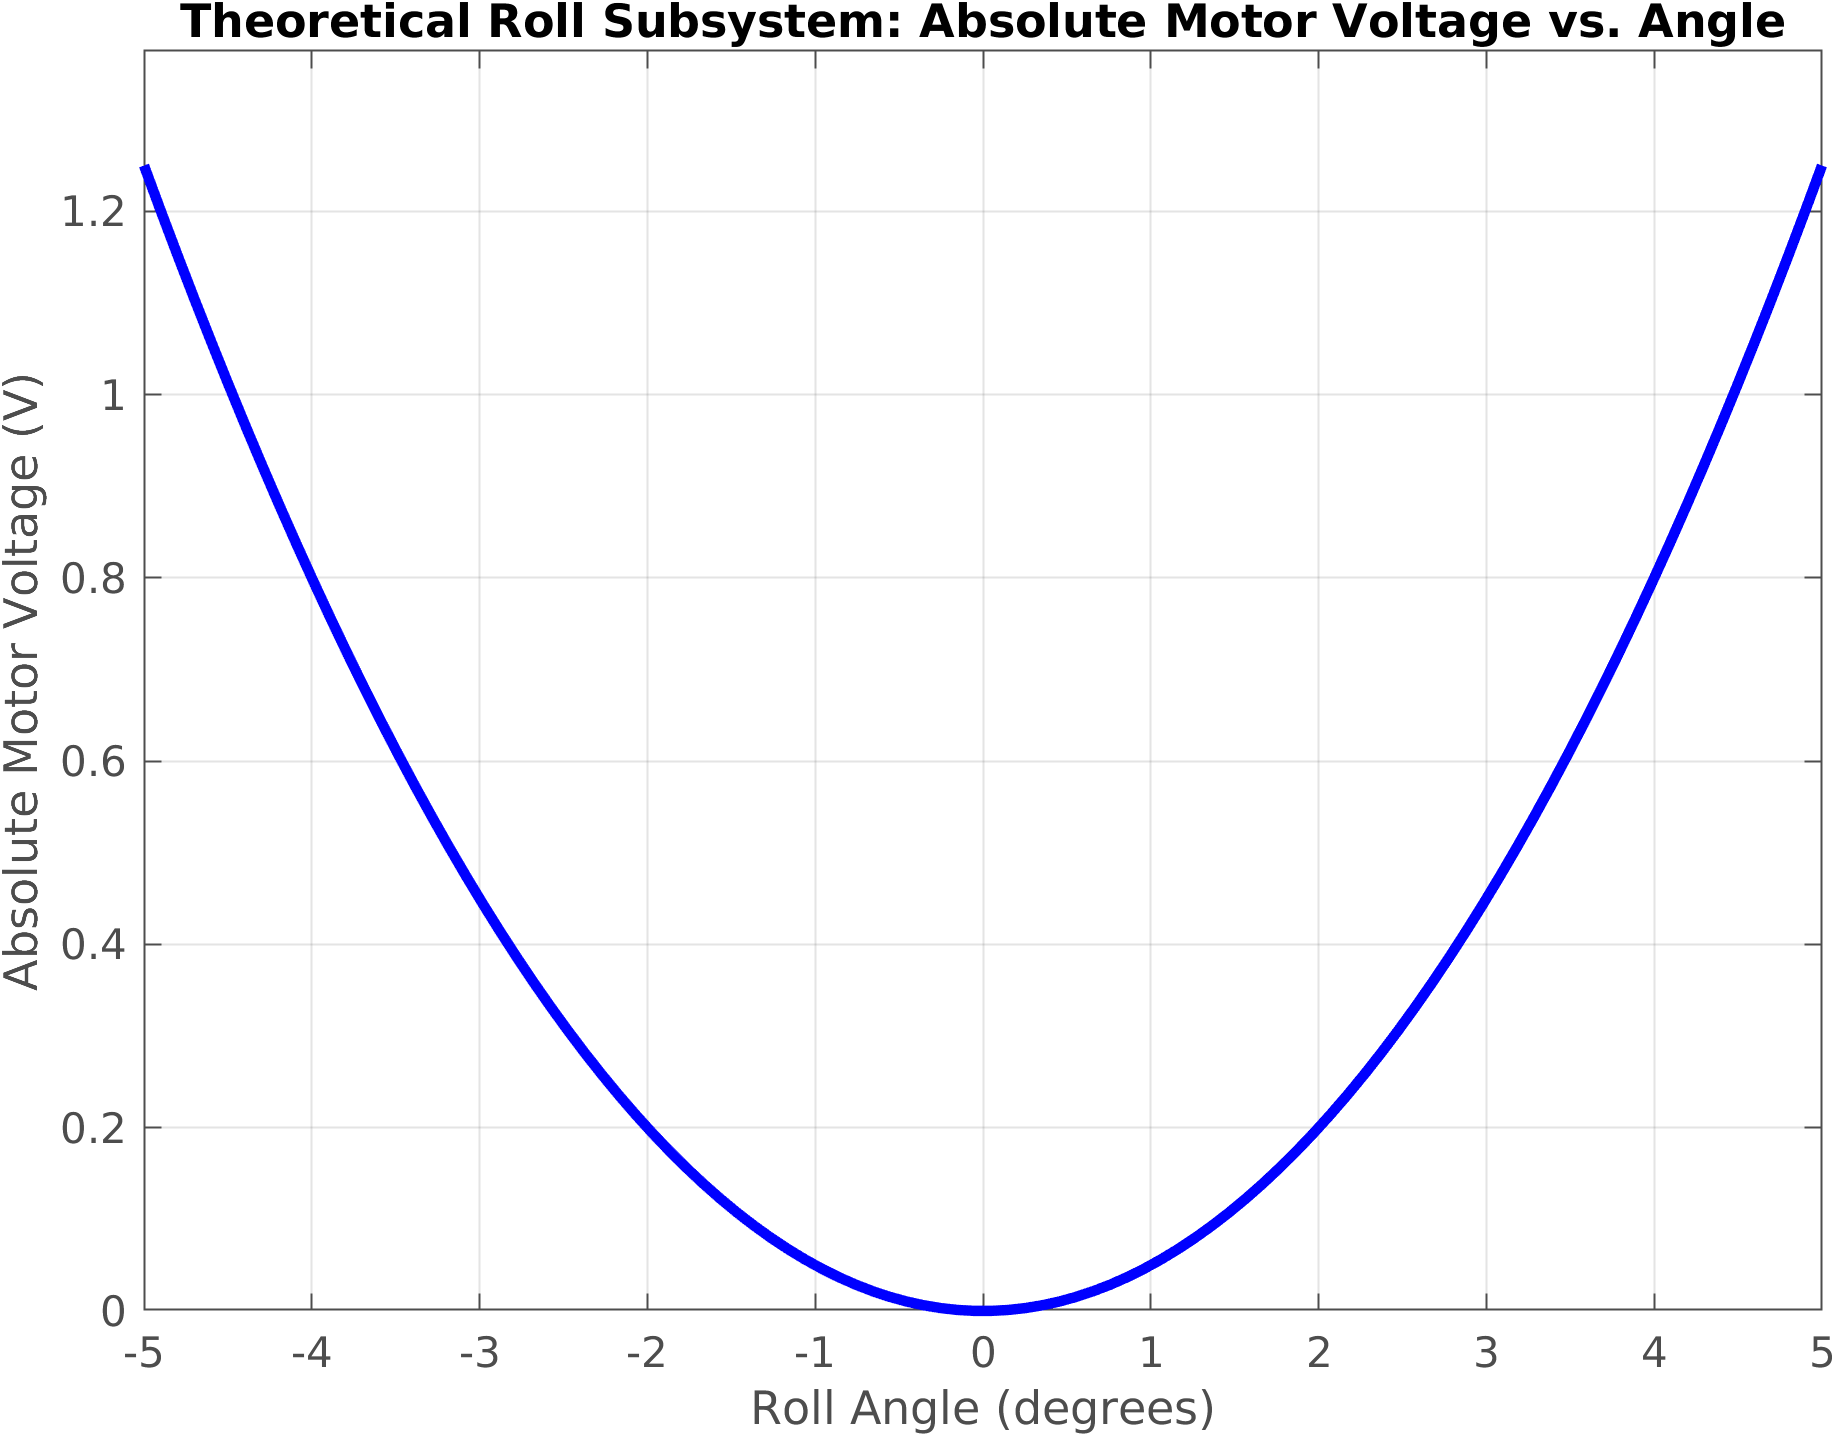
\includegraphics[width=0.7\textwidth]{figures/Roll_Subsystem_Theoretical_Trend.png}
    \caption{Theoretical trend of absolute motor voltage required for the roll subsystem as a function of roll angle.}
    \label{fig:roll_voltage_trend}
\end{figure}


\begin{figure}[H]
    \centering
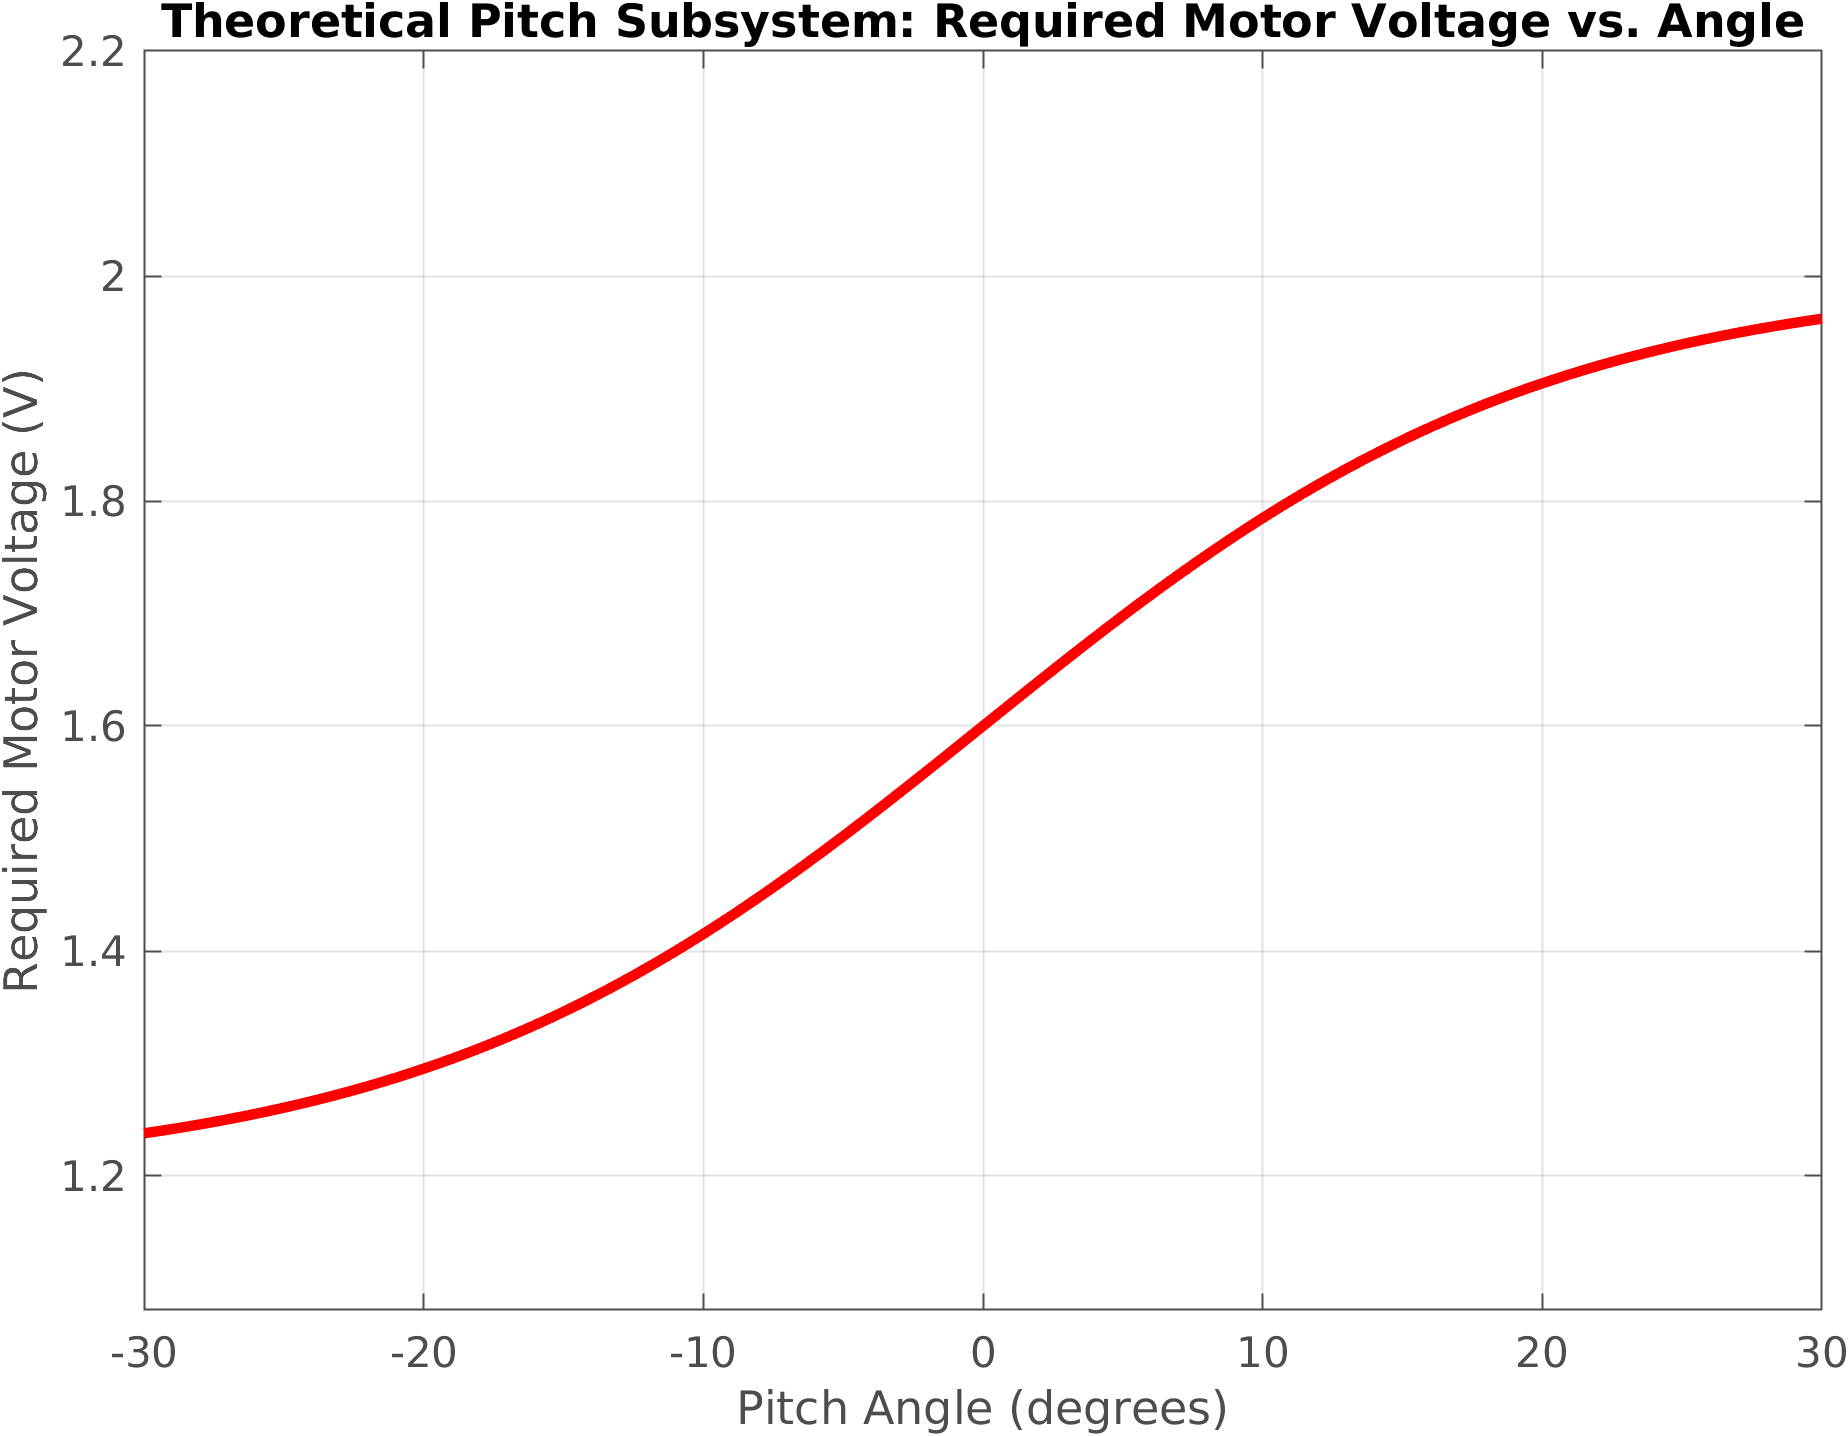
\includegraphics[width=0.75\textwidth]{figures/Pitch_Subsystem_Theoretical_Trend.png}
    \caption{Theoretical trend of required motor voltage for the pitch subsystem as a function of pitch angle.}
    \label{fig:pitch_voltage_trend}
\end{figure}

For the pitch subsystem, the force required by the actuator actually decreases as the joint moves through its range of motion from -30 degrees to 30 degrees. The theoretical voltage required for the pitch subsystem across its range of motion is shown in Figure~\ref{fig:pitch_voltage_trend}.


Additionally, complexities are added to the system dynamics when one realizes that the force required by the roll subsystem is also coupled to the pitch subsystem's position. As the pitch subsystem's angle is increased, the force required by the roll subsequently changes due to the system's center of mass changing position.

Similarly, the force required by the pitch subsystem varies with the position of the roll subsystem. As the roll subsystem diverges from the 0 point, the force required by the pitch subsystem lessens as it stays farther from its default position (normal to the gravitational force vector).

The combination of these factors necessitated the need for a more complex controller strategy in which the controller gains varied in accordance with the system position. The idea of this improved controller was that each joint's gains would vary with the current position of each subsystem.

This adaptive controller algorithm would require the characterization of the system at multiple points of the system's position. It was decided that 9 characterization points would be used for each joint of the subsystem. The pitch would be varied from $-15^\circ$, $0^\circ$, $15^\circ$ and the roll subsystem would vary from $-20^\circ$, $0^\circ$, $20^\circ$. This resulted in the following grid of 9 characterization points:

\begin{table}[htbp]
    \centering
    \caption{Grid of 9 Characterization Points for System Identification}
    \label{tab:characterization_points}
    \begin{tabular}{c|ccc} % c for the first column, then 3 c's for the data columns
        \multicolumn{1}{c}{} & \multicolumn{3}{c}{\textbf{Roll Angle ($^\circ$)}} \\
        \cmidrule(lr){2-4} % Line under Roll Angle
        \cmidrule(lr){1-1} % <<< MODIFIED: Line above Pitch Angle, similar to Roll Angle
        \textbf{Pitch Angle ($^\circ$)} & \textbf{-20} & \textbf{0} & \textbf{20} \\
        \midrule % Line separating headers from data
        \textbf{-15} & $(-15, -20)$ & $(-15, 0)$ & $(-15, 20)$ \\
        \textbf{0}    & $(0, -20)$    & $(0, 0)$    & $(0, 20)$    \\
        \textbf{15}   & $(15, -20)$  & $(15, 0)$  & $(15, 20)$  \\
        \bottomrule
    \end{tabular}
\end{table}

Once the necessary characterization points were established, the system needed to be identified at each of these points for each joint, resulting in the necessary system identification procedures. The actual system identification process was fairly straightforward. The previously established strategy for each joint was used; the only difference was that the positional setpoint for each characterization point varied to ensure the joint not being characterized remained at the necessary setpoint. The controller designed around the $(0,0)$ characterization point was used. While it was found that the dynamic performance of the controller designed around the $(0,0)$ setpoint degraded as the system diverged farther from the original linearization point, this controller performed well enough in the case of a static setpoint that it could be used to hold the extreme angles required by the multi-point system identification.

Once the necessary characterization points were established, the system needed to be identified at each of these points for each joint, resulting in the necessary system identification procedures. The actual system identification process was fairly straightforward. The previously established strategy for each joint was used; the only difference was that the positional setpoint for each characterization point varied to ensure the joint not being characterized remained at the necessary setpoint. The controller designed around the $(0,0)$ characterization point was used. While it was found that the dynamic performance of the controller designed around the $(0,0)$ setpoint degraded as the system diverged farther from the original linearization point, this controller performed well enough in the case of a static setpoint that it could be used to hold the extreme angles required by the multi-point system identification.

Upon the completion of each system identification trial, the resulting system response was saved in a CSV file under the following format: \texttt{IDENTIFIEDJOINT\_ROLLANGLE\_PITCHANGLE.csv}. A MATLAB script was then used to parse each of these files, identify the system at that point, and store and plot the system identification results.

The specific implementation of the multi-point system identification for the roll joint is as follows:

\textbf{Data Loading and Preprocessing}
The raw sensor data is loaded from a CSV file. For the Roll system, a step response is analyzed. The data is then trimmed to isolate the relevant section around the step change, and normalized by subtracting initial values to focus on the system's response to the step input.

\begin{figure}[h!]
\centering
\begin{lstlisting}[caption={Roll Data Loading and Preprocessing}, label={lst:roll_data_prep}]
% Read CSV file with preserved headers
roll_data = readtable('roll_step.csv', 'VariableNamingRule', 'preserve');
% Extract time and normalize
roll_time = roll_data.time - roll_data.time(1);
% Extract roll data using original column names
roll_position = roll_data.('roll_position');
roll_velocity = roll_data.('roll_velocity');
roll_effort = roll_data.('roll_effort');

% Find step change time and trim data
velocity_threshold = 0.1;
roll_step_idx = find(abs(diff(roll_velocity)) > velocity_threshold, 1);
roll_trim_idx = roll_step_idx:min(roll_step_idx+500, length(roll_time));

% Prepare data for system ID (normalize to start from zero)
roll_y = roll_position(roll_trim_idx) - roll_position(roll_trim_idx(1));
roll_t = roll_time(roll_trim_idx) - roll_time(roll_trim_idx(1));
roll_u = roll_velocity(roll_trim_idx) - roll_velocity(roll_trim_idx(1));
\end{lstlisting}
\end{figure}

\textbf{System Identification (Transfer Function Estimation)}
Next, a 2nd-order transfer function is estimated from the preprocessed input-output data using the \texttt{tfest} function. The \texttt{iddata} object encapsulates the input, output, and sampling time.

\begin{figure}[h!]
\centering
\begin{lstlisting}[caption={Roll Transfer Function Estimation}, label={lst:roll_tfest}]
% Prepare data for system ID
roll_data_iddata = iddata(roll_y, roll_u, mean(diff(roll_t)));
% Fit transfer function (2nd-order)
roll_sys = tfest(roll_data_iddata, 2);
\end{lstlisting}
\end{figure}
The estimated transfer function \texttt{roll\_sys} is then converted to a state-space representation (\texttt{roll\_ss\_sys}) to facilitate LQR design.

\textbf{State-Space Matrix Extraction and Controllability Check}
After obtaining the transfer function, it is converted into a state-space representation. This form provides the system matrices (\texttt{A}, \texttt{B}, \texttt{C}, \texttt{D}) which are essential for designing state-feedback controllers like LQR. The controllability is than checked by examining the rank of the controllability matrix.

\begin{figure}[h!]
\centering
\begin{lstlisting}[caption={Roll State-Space Extraction and Controllability Check}, label={lst:roll_statespace_controllability}]
% Convert to state-space
roll_ss_sys = ss(roll_sys);
roll_A = roll_ss_sys.A;
roll_B = roll_ss_sys.B;
roll_C = roll_ss_sys.C;
roll_D = roll_ss_sys.D;
% Check controllability
if rank(ctrb(roll_A, roll_B)) == size(roll_A, 1)
    disp('Roll System is controllable');
else
    error('Roll System is uncontrollable! Check model.');
end
\end{lstlisting}
\end{figure}
\section{Controller Design}

After system identification was performed, a controller can be designed for the specific system. The controller design was paramount to this research; a high emphasis was placed on system performance, and proper controller design would directly drive this. As a result, a large amount of effort was put into both the design and tuning of the controller.

\subsection{Original PID Controller}

The system originally utilized a very basic PID controller. Tuning was conducted with the Ziegler-Nichols method, and the following gains were found for each subsystem:

\begin{table}[htbp]
    \centering
    \caption{Ziegler-Nichols PID Gains for Roll and Pitch Subsystems}
    \label{tab:pid_gains}
    \begin{tabular}{l c c c}
        \toprule
        \textbf{Subsystem} & \textbf{$k_p$} & \textbf{$k_i$} & \textbf{$k_d$} \\
        \midrule
        Roll               & 35             & 50             & 5              \\
        Pitch              & 60             & 110            & 5              \\
        \bottomrule
    \end{tabular}
\end{table}

However, with these values, when full PID control was used, the system would rapidly vibrate, leading to uncontrolled system behavior and unacceptable noise and vibration. Because of this, the original system was only ever used with PD control, and its performance suffered greatly. Following sinusoidal trajectories, it would frequently undershoot or overshoot the setpoint and responded poorly to perturbations. As a result, an improved controller method needed to be developed.


\subsection{Model Predictive Control}

Initially, several types of controllers were considered for this system. Model Predictive Control (MPC) was initially considered, as the system was already partially modeled in the form of an SDF model. MPC uses a dynamic model of the system to predict system behavior and determine a cost-optimal control input based on the model dynamics. While this control technique would result in extremely robust and optimal control, two factors prevented its utilization. First, the system model was a purely geometrical model, only accounting for the mass and inertia properties. Internal dynamics, such as frictional forces, were not considered, and the complexities of modeling such behavior were daunting. Secondly, MPC requires high computational power to simultaneously run and predict the model's behavior. This system utilized low-cost hardware with limited computational resources and, as a result, lacked the computational power to perform MPC.

\subsection{Gain Scheduling and Adaptive Control}

It was clear that due to varying system dynamics across the system's range of motion, adaptive control or gain scheduling would be a very valuable asset for improving system performance. Adaptive control involves online estimation of unknown or time-varying system parameters, or direct adjustment of controller parameters based on real-time performance feedback. In contrast, gain scheduling is a pre-programmed approach where controller parameters are adjusted based on a known, measurable "scheduling variable."

With relatively little additional computational power and complexity, the control gains could be calculated and interpolated based on the system's position, making gain scheduling an excellent candidate for improving system performance.

After the previously discussed multi-point system identification, a set of gains was calculated for each characterization point. These gains were then stored in tables, and the controller would interpolate between these gains based on the current position of the system using the following code.

\begin{figure}[h!]
    \centering
    \begin{lstlisting}[language=C++, caption={Linear Interpolation for Gain Scheduling}, label={lst:gain_interpolation}]
    // === Linear interpolation between two values ===
    double interpolate(double x, double x0, double x1, double y0, double y1) {
        return y0 + (y1 - y0) * ((x - x0) / (x1 - x0));
    }
    \end{lstlisting}
    \end{figure}

The gains used for the roll and pitch subsystems are presented in \autoref{tbl:kp_roll}, \autoref{tbl:kd_roll}, \autoref{tbl:kp_pitch}, \autoref{tbl:kd_pitch}, and \autoref{tbl:ki_pitch}. These gains were calculated based on the system identification results and were tuned to achieve optimal performance at each characterization point.

\begin{table}[H]
    \centering
    \caption{Roll Proportional Gain ($K_p$) Table}
    \label{tbl:kp_roll}
    \begin{tabular}{cccc} % Changed from {|c|c|c|c|}
    \toprule % Changed from \hline
    \textbf{Pitch / Roll} & \textbf{-15} & \textbf{0} & \textbf{15} \\
    \midrule % Changed from \hline
    \textbf{Pitch = -20} & 135.41 & 135.41 & 137.91 \\
    \textbf{Pitch = 0}   & 136.23 & 132.23 & 130.12 \\
    \textbf{Pitch = +20} & 137.36 & 135.77 & 131.78 \\
    \bottomrule % Changed from \hline
    \end{tabular}
    \end{table}
    
    \begin{table}[H]
    \centering
    \caption{Roll Derivative Gain ($K_d$) Table}
    \label{tbl:kd_roll}
    \begin{tabular}{cccc} % Changed from {|c|c|c|c|}
    \toprule % Changed from \hline
    \textbf{Pitch / Roll} & \textbf{-15} & \textbf{0} & \textbf{15} \\
    \midrule % Changed from \hline
    \textbf{Pitch = -20} & 0.6527 & 1.0829 & 0.43766 \\
    \textbf{Pitch = 0}   & 0.6854 & 0.7588 & 0.4810 \\
    \textbf{Pitch = +20} & 0.6579 & 1.0788 & 0.42543 \\
    \bottomrule % Changed from \hline
    \end{tabular}
    \end{table}
    
    \begin{table}[H]
    \centering
    \caption{Pitch Proportional Gain ($K_p$) Table}
    \label{tbl:kp_pitch}
    \begin{tabular}{cccc} % Changed from {|c|c|c|c|}
    \toprule % Changed from \hline
    \textbf{Pitch / Roll} & \textbf{-15} & \textbf{0} & \textbf{15} \\
    \midrule % Changed from \hline
    \textbf{Pitch = -20} & 188.07 & 195.37 & 191.11 \\
    \textbf{Pitch = 0}   & 161.41 & 166.32 & 167.01 \\
    \textbf{Pitch = +20} & 153.37 & 155.56 & 151.23 \\
    \bottomrule % Changed from \hline
    \end{tabular}
    \end{table}
    
    \begin{table}[H]
    \centering
    \caption{Pitch Derivative Gain ($K_d$) Table}
    \label{tbl:kd_pitch}
    \begin{tabular}{cccc} % Changed from {|c|c|c|c|}
    \toprule % Changed from \hline
    \textbf{Pitch / Roll} & \textbf{-15} & \textbf{0} & \textbf{15} \\
    \midrule % Changed from \hline
    \textbf{Pitch = -20} & 0.3124 & 0.3256 & 0.3154 \\
    \textbf{Pitch = 0}   & 0.3671 & 0.3671 & 0.3272 \\
    \textbf{Pitch = +20} & 0.3643 & 0.3374 & 0.3576 \\
    \bottomrule % Changed from \hline
    \end{tabular}
    \end{table}
    
    \begin{table}[H]
    \centering
    \caption{Pitch Integral Gain ($K_i$) Table}
    \label{tbl:ki_pitch}
    \begin{tabular}{cccc} % Changed from {|c|c|c|c|}
    \toprule % Changed from \hline
    \textbf{Pitch / Roll} & \textbf{-15} & \textbf{0} & \textbf{15} \\
    \midrule % Changed from \hline
    \textbf{Pitch = -20} & 0.143744 & 0.185649 & 0.164665 \\
    \textbf{Pitch = 0}   & 0.135649 & 0.153566 & 0.155123 \\
    \textbf{Pitch = +20} & 0.124432 & 0.155649 & 0.134566 \\
    \bottomrule % Changed from \hline
    \end{tabular}
    \end{table}

\subsection{LQR and LQI Control}

Linear Quadratic Regulator (LQR) control and Linear Quadratic Integral (LQI) control are cost-optimal control algorithms that minimize a quadratic cost function. LQI control extends the efforts of LQR control by incorporating integral action, which reduces steady-state error and improves system performance.

Both of these control methods are well-suited to this research as they achieve a good balance of high system performance with minimal control efforts. LQR control was chosen for the roll joint, as it was found that its performance was more than adequate for the system. However, during testing of the pitch subsystem, it was found that the system was consistently undershooting the desired positional setpoint. It was found that an LQI controller would minimize this steady-state error and drastically improve performance.

The objective of LQR control is to find a control input $\mathbf{u}(t)$ that minimizes the following quadratic cost function:
$$ J_{LQR} = \int_{0}^{\infty} (\mathbf{x}^T(t) Q \mathbf{x}(t) + \mathbf{u}^T(t) R \mathbf{u}(t)) \, dt $$
where:
\begin{itemize}
    \item $\mathbf{x}(t)$ is the state vector.
    \item $\mathbf{u}(t)$ is the control input vector.
    \item $Q$ is a weighting matrix for the states, penalizing deviations from the desired state
    \item $R$ is a weighting matrix for the control inputs, penalizing control effort.
\end{itemize}

For LQI control, the integral of the error is added to the system, and the cost function is also minimized. If $\mathbf{e}_I(t)$ represents the integral of the output error, the augmented state $\mathbf{x}_{aug}(t)$ includes the original states and the integral error. The cost function for LQI is then:
$$ J_{LQI} = \int_{0}^{\infty} (\mathbf{x}_{aug}^T(t) \tilde{Q} \mathbf{x}_{aug}(t) + \mathbf{u}^T(t) R \mathbf{u}(t)) \, dt $$
where $\tilde{Q}$ is the augmented weighting matrix for the states, including a penalty on the integral error to drive it to zero.

The specific Q and R matrices used for this controller were numerically determined by trial and error during the research to maximize system while maintaining stability. 

The following is a detailed implementation of the LQR and LQI controllers in the PSM software. 

\textbf{Roll LQR Controller Implementation}

The calculated LQR gains were input as a vector to the LQR control function along with the commanded position and the actual position. From here several key variables were initialized. The current time was determined and from this the $\Delta t$ value was calculated then used to calculate the actual velocity. A low-pass filter was then applied to this value. The velocity and positional error were then determined and the control input was calculated from these error values scaled by their respective gains $K_p$ and $K_d$. The implementation of this in the system software can be seen below.

\begin{figure}[H]
\centering
\begin{lstlisting}[caption={Roll LQR Control Input Calculation}, label={lst:roll_lqr_control}]
float compute_roll_LQR_control(float* gains, float commanded_position, float actual_position) {
    static float previous_position_roll = 0.0f;
    static unsigned long previous_time_roll = 0;
    static float filtered_velocity_roll = 0.0f;
    const float alpha = 0.9f;

    unsigned long current_time = micros();
    float delta_time = (current_time - previous_time_roll) / 1000000.0f;
    if (delta_time <= 0.0f) delta_time = 0.000001f;

    float raw_velocity = (actual_position - previous_position_roll) / delta_time;
    filtered_velocity_roll = alpha * filtered_velocity_roll + (1.0f - alpha) * raw_velocity;

    previous_position_roll = actual_position;
    previous_time_roll = current_time;

    float position_error = commanded_position - actual_position;
    float state[2] = {position_error, filtered_velocity_roll};

    float control_input = 0.0f;
    for (int i = 0; i < 2; i++) {
        control_input -= gains[i] * state[i];
    }

    return control_input;
}
\end{lstlisting}
\end{figure}

\textbf{Pitch LQI Controller Implementation (with Feedforward)}

The Pitch joint LQI controller implementation was very similar to the Roll joint LQR controller implementation. The function input a gain vector along with actual position and commanded positions. These values were then used to calculate the positional and velocity error values. The positional error was then multiplied by $\Delta t$ to calculate the integral error. These errors were scaled by their respective gain values and the control input before feedforward control was calculated. To calculate the feedforward control input component, the $B^\dagger$ matrix is multiplied by the sum of the system's $A$ matrix and the reference state. The $U_{ff}$ is then scaled by $\lambda$ and added to the original control input. The detailed software implementation can be seen below:

\begin{figure}[H]
\centering
\begin{lstlisting}[caption={Pitch LQI Control with Feedforward}, label={lst:pitch_lqi_control}]
float compute_pitch_LQI_control(float* gains, float commanded_position, float actual_position) {
    static float previous_position_pitch = 0.0f;
    static float previous_commanded_position_pitch = 0.0f;
    static unsigned long previous_time_pitch = 0;
    static float integral_error = 0.0f;
    const float lambda = 0.0f;

    const float A[2][2] = {{-4.3950, -2.3842}, {4.0000, 0.0}};
    const float B_dagger[2][2] = {{0.5, 0.0}, {0.0, 0.0}};

    unsigned long current_time = micros();
    float delta_time = (current_time - previous_time_pitch) / 1000000.0f;
    if (delta_time <= 0.0f) delta_time = 0.000001f;

    float raw_velocity = (actual_position - previous_position_pitch) / delta_time;
    previous_position_pitch = actual_position;
    previous_time_pitch = current_time;

    float position_error = commanded_position - actual_position;
    integral_error += position_error * delta_time;

    float state[3] = {position_error, raw_velocity, integral_error};

    float control_input = 0.0f;
    for (int i = 0; i < 3; i++) {
        control_input -= gains[i] * state[i];
    }

    float x_ref_dot = (commanded_position - previous_commanded_position_pitch) / delta_time;
    previous_commanded_position_pitch = commanded_position;

    float x_ref[2] = {commanded_position, x_ref_dot};
    float u_ff = 0.0f;
    for (int i = 0; i < 2; i++) {
        float Ax_ref = 0.0f;
        for (int j = 0; j < 2; j++) {
            Ax_ref += A[i][j] * x_ref[j];
        }
        u_ff += B_dagger[i][i] * (Ax_ref + x_ref_dot);
    }

    control_input += lambda * u_ff;

    return control_input;
}
\end{lstlisting}
\end{figure}

\subsection{Feedforward Control}

Feedforward control is a control method which attempts to anticipate changes or disturbances to the system's input. It was theorized that a feedforward control strategy could further reduce any remaining steady-state error in the pitch subsystem.

In order for feedforward control to be implemented, a model of the system must be constructed in the form of a specific matrix known as the $B^\dagger$ matrix. The $B^\dagger$ matrix is formulated through the Moore-Penrose pseudoinverse. It is formulated as follows:

Let $B$ be an $m \times n$ real or complex matrix. Its Singular Value Decomposition (SVD) is given by:
$$B = U \Sigma V^T$$
where:
\begin{itemize}
    \item $U$ is an $m \times m$ unitary (or orthogonal for real matrices) matrix whose columns are the left singular vectors of $B$.
    \item $\Sigma$ is an $m \times n$ rectangular diagonal matrix with non-negative real numbers on the diagonal, called the singular values of $B$, typically arranged in decreasing order.
    \item $V^T$ is an $n \times n$ unitary (or orthogonal for real matrices) matrix whose rows are the right singular vectors of $B$. ($V$ is the matrix of right singular vectors).
\end{itemize}

The \textbf{Moore-Penrose pseudoinverse} of $B$, denoted $B^\dagger$, is then defined as:
$$B^\dagger = V \Sigma^\dagger U^T$$
where $\Sigma^\dagger$ is an $n \times m$ matrix formed by taking the reciprocal of each non-zero singular value on the diagonal of $\Sigma$, and then transposing the matrix.



For the purpose of this research, this matrix could be calculated via the MATLAB command \texttt{pinv}. This command, when applied to the identified $B$ matrix from the system identification procedure, would result in the $B^\dagger$ matrix.


This procedure was conducted for each of the characterization points previously discussed. Upon calculation of the $B^\dagger$ matrix, this matrix is used to calculate $u_{ff}$ by multiplying the $B^\dagger$ matrix (pseudoinverse of the input matrix) with the sum of the system's $A$ matrix multiplied by the reference state and the time derivative of the reference state. This $u_{ff}$ is then scaled by a factor $\lambda$, which can be tuned from $0$ to $1.0$ to adjust the feedforward element of the controller.

The ultimate result of this control effort is to proactively cancel anticipated system dynamics and generate better system performance.

\subsection{Comprehensive Control Strategy}


The final controller for the system was a resulting combination of several of the control strategies previously discussed. Ultimately, for the roll joint, it was found that gain scheduling with an LQR controller provided adequate system performance. However, for the pitch subsystem, this method needed to be improved upon due to consistent steady-state error in the form of target undershooting. To remedy this, an LQI controller with feedforward implementation and gain scheduling was employed. These strategies led to drastic improvements in system performance.

\chapter{System evaluation}
\label{chapter:results}

In an effort to demonstrate the effectiveness of the designed control system, a robust evaluation procedure was developed. This procedure and its results will be explored in this section.


\section{Overview of Experiments}
\label{section:experiment_overview}

The evaluation of the control system was conducted through a series of experiments designed to assess its performance under various conditions. The experiments were structured to test the system's response to different trajectories. Two primary experiments were developed to evaluate this:

\begin{itemize}
    \item \textbf{Sinusoidal Path Following}: This experiment consisted of a pre-generated sinusoidal path that the robot was required to follow. The path was designed to test the system's ability to track a smooth, continuous trajectory while maintaining stability and accuracy. The period of the sine wave was chosen to test the system's response to rapid velocities, and its amplitude was selected to push the system towards its extrema in each axis. The following parameters were chosen for each axis:
    \begin{itemize}
        \item \textbf{Pitch Period}: 3 seconds
        \item \textbf{Pitch Amplitude}: $\pm 15$ degrees
        \item \textbf{Roll Period}: 3 seconds
        \item \textbf{Roll Amplitude}: $\pm 20$ degrees
    \end{itemize}
    
    \item \textbf{Target Following}: This experiment was designed to more accurately reflect real-world conditions that the subsystems would encounter in practice. The MTM was used to generate a target trajectory path that was representative of typical movements in a surgical procedure. Both axes then attempted to follow this path as closely as possible.
\end{itemize}

During these experiments, the improved control algorithm was tested alongside the previously developed control algorithm. During each trial, the target position, actual positions, commanded motor speed, and positional error were carefully tracked and logged. This data was then parsed using a custom MATLAB script and plotted to compare the performance of the two control algorithms. The following sections detail the results of these experiments, focusing on trajectory tracking performance and the effect of the control algorithm on the system's overall performance.

\section{Control Algorithm Performance}
\label{section:trajectory_performance}

These experiments revealed a significant increase in performance for the new control algorithm. It was observed during both the sinusoidal path-following and trajectory-following experiments that the positional error was greatly reduced in both the roll and pitch axes. With the previous proportional control algorithm, the system consistently undershot or overshot the target position and lagged behind the intended trajectory, particularly at the extrema of the joint angles.

With the proportional control algorithm, the error in the pitch axis reached a maximum value of 2.31 degrees, while the error in the roll axis reached 1.17 degrees. The overall average error for the pitch axis was VALUE HERE, and the overall average error for the roll axis was VALUE HERE. These errors were particularly pronounced at the extrema of the joint angles, where the system struggled to maintain accuracy and stability.

With the new LQR and LQI with feedforward control algorithm, the maximum error in the pitch axis was reduced to 0.35 degrees, and the maximum error in the roll axis was reduced to 0.41 degrees. Both of these errors occurred at the extreme limits of their respective axes, and the average error of the pitch axis over the trial was VALUE HERE while the value for the average error over the trial for the roll dof was VALUE HERE.

Overall, the performance of the new control algorithm greatly exceeded that of the old algorithm. It was found that the the overall positional error of the system was greatly  reduced and that the system no longer lagged behind or undershot the desiredd positional target. 
\chapter{Conclusion and Future Work}
\label{chapter:conclusion}


\section{Summary of Research Objectives}
\label{section:summary_objectives}

\section{Key Findings}
\label{section:key_findings}

\section{Limitations}
\label{section:limitations}

\section{Recommendations for Future Work}
\label{section:future_work}

\section{Final Remarks}
\label{section:final_remarks}

%\selectlanguage{english} % Re-select English if previous chapters were in German

% --- Listings (Code/Pseudo-code) ---
% Literaturverzeichnis IEEE-gerecht
\bibliographystyle{IEEEtran}	
\bibliography{bibliography}
\ifthenelse{\boolean{english}}{\addcontentsline{toc}{chapter}{Bibliography}}{\addcontentsline{toc}{chapter}{Literaturverzeichnis}} % f"ugt den Eintrag "Abbildungsverzeichnis" im Inhaltsverzeichnis hinzu

\pagenumbering{Roman}
\setcounter{page}{\value{romancount}}

\newpage

% Abbildungsverzeichnis
\listoffigures
\ifthenelse{\boolean{english}}{\addcontentsline{toc}{chapter}{List of Figures}}{\addcontentsline{toc}{chapter}{Abbildungsverzeichnis}} % f"ugt den Eintrag "Abbildungsverzeichnis" im Inhaltsverzeichnis hinzu
\newpage

% Tabellenverzeichnis
\listoftables 
\ifthenelse{\boolean{english}}{\addcontentsline{toc}{chapter}{List of Tables}}{\addcontentsline{toc}{chapter}{Tabellenverzeichnis}} % f"ugt den Eintrag "Tabellenverzeichnis" im Inhaltsverzeichnis hinzu
\newpage



 % Includes code listings or similar content

% --- Appendices ---
\begin{appendix} % Starts the appendix section
    
\end{figure} % Includes MATLAB-related appendix content
    \input{appendix/Jupyter} % Includes Jupyter-related appendix content
\end{appendix}

\end{document}